\documentclass[12pt,pdflatex]{elsarticle} 
% this is edited by MDW to try to get to the 10000 word limit
% November 2, 2016
%%%%%%%%%%%%%%%%%%%%%%%%%%%%%%%%%%%%%%%%%%%%%%%%%%
%%%%%%%%%%%%%%%%%%%% PREAMBLE %%%%%%%%%%%%%%%%%%%%
%%%%%%%%%%%%%%%%%%%%%%%%%%%%%%%%%%%%%%%%%%%%%%%%%%


% -------------------- defaults -------------------- %
% load lots o' packages

% references
\usepackage{natbib}

% Fonts
\usepackage[default,osfigures,scale=0.95]{opensans}
\usepackage[T1]{fontenc}
\usepackage{ae}
% to colorize links in document. See color specification below
\usepackage[pdftex,hyperref,x11names]{xcolor}
% load the hyper-references package and set document info
\usepackage[pdftex]{hyperref}

% Generate some fake text
\usepackage{blindtext}

% layout control
\usepackage{geometry}
\geometry{verbose,tmargin=1.25in,bmargin=1.25in,lmargin=1.1in,rmargin=1.1in}
\usepackage{parallel}
\usepackage{parcolumns}
\usepackage{fancyhdr}

% math typesetting
\usepackage{array}
\usepackage{amsmath}
\usepackage{amssymb}
\usepackage{amsfonts}
\usepackage{relsize}
\usepackage{mathtools}
\usepackage{bm}
\usepackage[%
decimalsymbol=.,
digitsep=fullstop
]{siunitx}

% restricts float objects to be inserted before end of section
% creates float barriers
\usepackage[section]{placeins}

% tables
\usepackage{tabularx}
\usepackage{booktabs}
\usepackage{multicol}
\usepackage{multirow}
\usepackage{longtable}

% to adapt caption style
\usepackage[font={small},labelfont=bf]{caption}

% footnotes at bottom
\usepackage[bottom]{footmisc}

% to change enumeration symbols begin{enumerate}[(a)]
\usepackage{enumerate}

% to make enumerations and itemizations within paragraphs or
% lines. f.i. begin{inparaenum} for (a) is (b) and (c)
\usepackage{paralist}

% graphics stuff
\usepackage{subfig}
\usepackage{graphicx}
\usepackage[space]{grffile} % allows us to specify directories that have spaces
\usepackage{placeins} % prevents floats from moving past a \FloatBarrier
\usepackage{tikz}
\usepackage{rotating}

% Spacing
\usepackage[singlespacing]{setspace}

% -------------------------------------------------- %


% -------------------- page template -------------------- %

\setlength{\headheight}{15pt}
\setlength{\headsep}{20pt}
\pagestyle{fancyplain}
 
\fancyhf{}
 
\lhead{\fancyplain{}{}}
\chead{\fancyplain{}{Amen for LFM}}
\rhead{\fancyplain{}{\today}}
\rfoot{\fancyplain{}{\thepage}}

% ----------------------------------------------- %


% -------------------- customizations -------------------- %

% easy commands for number propers
\newcommand{\first}{$1^{\text{st}}$}
\newcommand{\second}{$2^{\text{nd}}$}
\newcommand{\third}{$3^{\text{rd}}$}
\newcommand{\nth}[1]{${#1}^{\text{th}}$}

% easy command for boldface math symbols
\newcommand{\mbs}[1]{\boldsymbol{#1}}

% command for R package font
\newcommand{\pkg}[1]{{\fontseries{b}\selectfont #1}}

% approx iid
\newcommand\simiid{\stackrel{\mathclap{\normalfont\mbox{\tiny{iid}}}}{\sim}}

% -------------------------------------------------------- %

%%%%%%%%%%%%%%%%%%%%%%%%%%%%%%%%%%%%%%%%%%%%%%%%%%
%%%%%%%%%%%%%%%%%%%% DOCUMENT %%%%%%%%%%%%%%%%%%%%
%%%%%%%%%%%%%%%%%%%%%%%%%%%%%%%%%%%%%%%%%%%%%%%%%%

% remove silly elsevier preprint note
\makeatletter
\def\ps@pprintTitle{%
 \let\@oddhead\@empty
 \let\@evenhead\@empty
 \def\@oddfoot{}%
 \let\@evenfoot\@oddfoot}

\def\input@path{{/Users/janus829/Dropbox/Research/netModels/summResults/}, {/Users/s7m/Dropbox/Research/netModels/summResults/}, {/Users/mdw/Dropbox/netModels/summResults/}}
\graphicspath{{/Users/janus829/Dropbox/Research/netModels/summResults/}, {/Users/s7m/Dropbox/Research/netModels/summResults/},{/Users/mdw/Dropbox/netModels/summResults/}}
\makeatother

\begin{document}

% % saying hello ----------------------------------------------- %
% \thispagestyle{empty}
% \begin{frontmatter}
%
% \title{Inferential Approaches for Network Analysis: \\ AMEN for Latent Factor Models\tnoteref{t1}}
%
% \tnotetext[t1]{This research was partially supported by the National Science Foundation Award 1259266.}
%
% \author[duke]{Shahryar Minhas\corref{cor1}}
% \ead{shahryar.minhas@duke.edu}
% \cortext[cor1]{Corresponding author}
% \author[duke2]{Peter D. Hoff}
% \author[duke]{Michael D. Ward}
%
% \address[duke]{Department of Political Science, Duke University, Durham, NC 27701, USA}
% \address[duke2]{Departments of Statistics, Duke University, Durham, NC 27701, USA}
%
% % \begin{abstract}
% %  Many network approaches have been developed in descriptive fashion, but attention to inferential approaches to network analysis has been growing. We introduce a new approach that models interdependencies among observations using additive and multiplicative effects (AME). This approach can be applied to binary, ordinal, and continuous network data, and provides a set of tools for inference from longitudinal networks as well. We review this approach and compare it to those examined in the recent survey by Cranmer et al. (2016).  The AME approach is shown a) to be easy to implement; b) interpretable in a general linear model framework; c) computationally straightforward; d) not prone to degeneracy; e) captures 1st, 2nd, and 3rd order network dependencies; and f) notably outperforms multiple regression quadratic assignment procedures, exponential random graph models, and alternative latent space approaches on a variety of metrics both in- and out-of-sample.
% % \end{abstract}
%
% \end{frontmatter}
% % ----------------------------------------------- %

\newpage\setcounter{page}{1} 

Network analysis provides a way to represent and study ``relational data'' with characteristics extending beyond those of the individual.   Data structures that extend beyond the country level are quite simply the norm in international relations. The dominant paradigm in  international relations for dealing with such data structures, however, is not a network approach but rather a dyadic design, in which an interaction between a pair of countries is considered independent of interactions between any other pair in the system.%\footnote{To highlight the ubiquity of this approach the following represent just a sampling of the articles published from the 1980s to the present in the American Journal of Political Science (AJPS) and American Political Science Review (APSR) that assume dyadic independence: \citet{dixon:1983,mansfield:etal:2000,lemke:reed:2001a,mitchell:2002,dafoe:2011a,fuhrmann:sechser:2014,carnegie:2014}.} 

The implication of this assumption is that when, for example, Vietnam and the United States decide to form a trade agreement, they make this decision independently of what they have done with other countries and what other countries in the international system have done among themselves.\footnote{There has been plenty of work done on treaty formation that would challenge this claim, e.g., see \citet{manger:etal:2012,kinne:2013}.} An even stronger assumption is that Japan declaring war against the United States is independent of the decision of the United States to go to war against Japan.
%\footnote{\citet{maoz:etal:2006,ward:etal:2007} would each note the importance of taking into account network dynamics in the study of interstate conflict.} 
A common defense of the dyad-only approach is that many events are only bilateral \citep{diehl:wright:2016}, thus alleviating the need for an approach that incorporates interdependencies between observations. This is clearly wrong. The network perspective asserts that even bilateral events and processes take place within a broader system. What takes place in one part of the system may be dependent upon events in another. At a minimum, we don't know whether independence of events and processes characterizes what we observe. We should at least examine this assertion.  

The potential for interdependence among observations poses a challenge to theoretical as well as statistical modeling since the assumption made by standard approaches used across the social sciences is that observations are, at least, conditionally independent \citep{snijders:2011}. The consequence of ignoring this assumption has been frequently noted within the political science literature already.\footnote{For example, see \citet{beck:etal:1998,signorino:1999,hoff:ward:2004,erikson:pinto:2014}.}  Just as relevant is the fact that a wealth of research from other disciplines suggests that carrying the independence assumption into a study with relational data is misguided and most often leads to biased inferences.%\footnote{From Computer Science see: \citet{bonabeau:2002,brandes:erlebach:2005}. From Economics see: \citet{goyal:2012,jackson:2014}. From Psychology see: \citet{pattison:wasserman:1999,kenny:etal:2006}. From Statistics and Sociology see: \citet{snijders:1996,hoff:etal:2002}.} 

Despite the hesitation among some in the discipline to adopt network analytic approaches, in recent years there has been a greater level of interest in understanding these approaches. For instance, in the past year a special issue focused on the application of a variety of network approaches has come out in the \textit{Journal of Peace Research}. Particularly notable is a recent overview and comparison of a handful of network based inferential models by \citet{cranmer:etal:2016}.
Specifically, they focus on the exponential random graph model (ERGM), the multiple regression quadratic assignment procedure (MRQAP), and a latent distance approach developed by \citet{hoff:etal:2002}. However, their discussion overlooks more than a decade worth of developments.\footnote{Indeed, in so far as we can tell, very few in political science have actually employed the Euclidean approach they summarize.} The principal latent variable approach used in political science has been the general bilinear mixed-effects (GBME) model developed by \citet{hoff:2005}. Examples of political science applications of the GBME model include \citet{ward:etal:2007,cao:2012,breunig:etal:2012,metternich:etal:2015,greenhill:2015}.%\footnote{The code necessary to run the GBME has been available since 2004 at the following address: \url{http://www.stat.washington.edu/people/pdhoff/Code/hoff_2005_jasa/}.} 
We are aware of only one political science application using the latent distance approach  \citep{kirkland:2012}. As \citet{hoff:2008} shows both empirically and mathematically, the distinction between the latent distance and latent factor models, such as the GBME model, is consequential when accounting for higher-order interdependencies, a point overlooked by Cranmer et al. (2016).

In this article, we introduce the additive and multiplicative effects model (AME). To highlight the benefits of this approach, we estimate this model using data from  the application presented in \citet{cranmer:etal:2016} and compare it to the other models presented in that article. By doing so we are able to show that AME provides a superior goodness of fit to the data than alternative approaches.\footnote{The AME approach has been developed into an $\sf{R}$ package named \pkg{amen} and is available on \href{https://cran.r-project.org/web/packages/amen/index.html}{CRAN} \citep{hoff:etal:2015}. \citet{hoff:2015:arxiv} provides a vignette for this package as well.} Further, through the AME approach we can estimate many different types of cross-sectional and longitudinal relational data (e.g., binomial, gaussian, and ordinal edges) in a straightforward way. 
%The rest of this article proceeds as follows: We briefly motivate the need for network oriented approaches; introduce the AME modeling framework; compare it to previous implementations of latent variable approaches; and then end by showing how this approach fits the application presented in \citet{cranmer:etal:2016}. 
The AME modeling framework  provides a flexible framework to study relational data. It addresses the issue of interdependence while still allowing scholars to examine theories that may only be relevant in the monadic or dyadic level. It accounts for both nodal and dyadic dependence patterns, and can include higher-order dependencies. 

\section{\textbf{Addressing Dependencies in Dyadic Data}}

Relational, or dyadic, data provide measurements of how pairs of actors relate to one another. 
%These structures encompass events of interest as diverse as the level of trade between countries $i$ and $j$ to the occurrence of an interstate conflict. 
The easiest way to organize such data is the directed dyadic design in which the unit of analysis is some set of $n$ actors that have been paired together to form a dataset of $z$ directed dyads. A tabular design such as this for a set of $n$ actors, $\{i, j, k, l \}$ results in $n \times (n-1)$ observations, as shown in Table~\ref{tab:canDesign}. 

\begin{table}[ht]
	\captionsetup{justification=raggedright }
	\centering
	\begin{minipage}{.45\textwidth}
		\centering
		\begingroup
		\setlength{\tabcolsep}{10pt}
		\begin{tabular}{ccc}
			Sender & Receiver & Event \\
			\hline\hline
			$i$ & $j$ & $y_{ij}$ \\
			\multirow{2}{*}{\vdots} & $k$ & $y_{ik}$ \\
			~ & $l$ & $y_{il}$ \\
			$j$ & $i$ & $y_{ji}$ \\
			\multirow{2}{*}{\vdots} & $k$ & $y_{jk}$ \\
			~ & $l$ & $y_{jl}$ \\
			$k$ & $i$ & $y_{ki}$ \\
			\multirow{2}{*}{\vdots} & $j$ & $y_{kj}$ \\
			~ & $l$ & $y_{kl}$ \\
			$l$ & $i$ & $y_{li}$ \\
			\multirow{2}{*}{\vdots} & $j$ & $y_{lj}$ \\
			~ & $k$ & $y_{lk}$ \\
			\hline\hline
		\end{tabular}
		\endgroup
		\caption{Structure of datasets used in canonical design.} 
		\label{tab:canDesign}
	\end{minipage}
	$\mathbf{\longrightarrow}$
	\begin{minipage}{.45\textwidth}
		\centering
		\begingroup
		\setlength{\tabcolsep}{10pt}
		\renewcommand{\arraystretch}{1.5}
		\begin{tabular}{c||cccc}
		~ & $i$ & $j$ & $k$ & $l$ \\ \hline\hline
		$i$ & \footnotesize{NA} & $y_{ij}$ & $y_{ik}$ & $y_{il}$ \\
		$j$ & $y_{ji}$ & \footnotesize{NA}  & $y_{jk}$ & $y_{jl}$ \\
		$k$ & $y_{ki}$ & $y_{kj}$ & \footnotesize{NA}  & $y_{kl}$ \\
		$l$ & $y_{li}$ & $y_{lj}$ & $y_{lk}$ & \footnotesize{NA}  \\
		\end{tabular}
		\endgroup
		\caption{Adjacency matrix representation of data in Table~\ref{tab:canDesign}. Senders are represented by the rows and receivers by the columns. }
		\label{tab:netDesign}
	\end{minipage}
\end{table}

\subsection{Limitations of the Standard Framework}

When modeling relational data, scholars typically employ a generalized linear model (GLM). This type of model is typically expressed via a stochastic and systematic component.
% \citep{pawitan:2013}. 
The stochastic component reflects assumptions about the probability distribution from which the data are generated: $y_{ij} \sim P(Y | \theta_{ij})$, with a probability density or mass function such as the normal, binomial, or Poisson. Each dyad in the sample is independently drawn from a particular distribution, given $\theta_{ij}$. The systematic component characterizes the model for the parameters of that distribution and describes how $\theta_{ij}$ varies as a function of a set of nodal and dyadic covariates, $\mathbf{X}_{ij}$: $\theta_{ij} = \bm\beta^{T} \mathbf{X}_{ij}$. A fundamental assumption we make when applying this modeling technique is that given $\mathbf{X}_{ij}$ and the parameters of the distribution, each of the dyadic observations is conditionally independent. 

The importance of this assumption becomes clearer in the process of estimating a GLM via maximum likelihood. After having chosen a set of covariates and specifying a distribution, the joint density function over all dyads using the observations from Table 1 is given:

\vspace{-8mm}
\begin{align}
\begin{aligned}
	P(y_{ij}, y_{ik}, \ldots, y_{lk} | \theta_{ij}, \theta_{ik}, \ldots, \theta_{lk}) &= P(y_{ij} | \theta_{ij}) \times P(y_{ik} | \theta_{ik}) \times \ldots \times P(y_{lk} | \theta_{lk}) \\
	P(\mathbf{Y} \; | \; \bm{\theta}) &= \prod_{\alpha=1}^{n \times (n-1)} P(y_{\alpha} | \theta_{\alpha})  \\
\end{aligned}
\end{align}

\noindent The joint probability is converted into a likelihood: $\displaystyle \mathcal{L} (\bm{\theta} | \mathbf{Y}) = \prod_{\alpha=1}^{n \times (n-1)} P(y_{\alpha} | \theta_{\alpha})$.

The parameters are estimated by maximizing the likelihood. The likelihood as defined above is only valid if  $y_{ij}$ is independent of $y_{ji}$ and $y_{ik}$ given the set of covariates we specified, or the values of $\theta_{ij}$.
%\footnote{The difficulties of applying the GLM framework to data that have structural interdependencies between observations is a problem that has long been recognized. \citet{beck:katz:1995} detail the issues with pooling observations in time-series cross-section datasets. \citet{ward:gleditsch:2008} have done the same in the case of spatial dependence.}
 Assuming that the dyad $y_{ij}$ is conditionally independent of the dyad $y_{ji}$ asserts that there is no level of reciprocity in a dataset, an assumption that in many cases would seem quite untenable.
 %\footnote{For example, see \citet{ward:etal:2007,cranmer:2014,dorff:minhas:2016}.} 
 A harder problem to handle is the assumption that $y_{ij}$ is conditionally independent of $y_{ik}$, the difficulty here follows from the possibility that $i$'s relationship with $k$ is dependent on how $i$ relates to $j$ and how $j$ relates to $k$, or more simply put the ``enemy of my enemy [may be] my friend''. 

The presence of these types of interdependencies in relational data complicates the \textit{a priori} assumption of observational independence. Without this assumption the joint density function cannot be written in the way described above and  a valid likelihood does not exist.\footnote{This problem has been noted in works such as \citet{lai:1995,manger:etal:2012,kinne:2013}.} Accordingly, inferences drawn from misspecified models that ignore potential interdependencies between dyadic observations are likely to have a number of issues including biased estimates of the effect of independent variables, uncalibrated confidence intervals, and poor predictive performance.\footnote{In cases where there is only ``dyadic clustering'' and no higher-order network effects such as transitivity, \citet{aronow:etal:2015} show that a nonparametric, variance estimator can be used to deal with the statistical issues that arise when working with dyadic data.} By ignoring these interdependencies, we ignore a potentially important part of the data generating process behind relational data, namely, network phenomena. 

\subsection{Social Relations Regression Model: Additive Part of AME}

The dependencies that tend to develop in relational data can be more easily understood when we move away from stacking dyads on top of one another and turn instead to adjacency matrices as shown in Table~\ref{tab:netDesign}. Operationally, this type of data structure is represented as a $n \times n$ matrix, $\mathbf{Y}$, where the diagonals in the matrix are typically undefined.
%\footnote{Most of the relational variables studied in political science do not involve events that countries can send to themselves.} 
The $ij^{th}$ entry defines the relationship between $i$ and $j$ and can be continuous or discrete. For example, in undirected data an event cannot be attributed to a specific sender or receiver rather it is just an indication of something that happened between a pair of countries or a relationship they share (e.g., two countries might have mutually agreed to form an alliance). If the relationship is undirected, the $ji^{th}$ entry will equal the $ij^{th}$ entry. Sociomatrices of directed relations are not symmetric, there is a specific sender and receiver, as in the case of bilateral or multilateral aid.

A common type of structural interdependency that arises in relational data is ``preferential attachment'' \citep{barabasi:reka:1999}. This is typically categorized as a first-order, or nodal, dependency and represents the fact that we typically find significant heterogeneity in activity levels across nodes. The implication of this across-node heterogeneity is within-node heterogeneity of ties, meaning that values across a row, say $\{y_{ij},y_{ik},y_{il}\}$, will be more similar to each other than other values in the adjacency matrix because each of these values has a common sender $i$. This type of dependency manifests in cases where sender $i$ tends to be more active or less active in the network than other senders. The emergence of this type of structure often occurs in relational datasets such as trade and conflict. In both of these cases, there are a set of countries that tend to be more active than others. Similarly, while some actors may be more active in sending ties to others in the network, we might also observe that others are more popular targets, this would manifest in observations down a column, $\{y_{ji},y_{ki},y_{li}\}$, being more similar. Last, we might also find that actors who are more likely to send ties in a network are also more likely to receive them, meaning that the row and column means of an adjacency matrix may be correlated. First-order dependencies are equally important to take into account in undirected relational structures, the only difference being that nodal heterogeneity will be equivalent across rows and columns. The presence of this type of heterogeneity in directed and undirected relational data leads to a violation of the conditional independence assumption underlying the models in our standard tool-kit, but can be easily accommodated in the GLM framework with the inclusion of additive sender and receiver random effects.
%\footnote{It can lead to so-called power law dynamics, which has reinforced the popularity of the assumption of preferential attachment in network studies.}

Another ubiquitous type of structural interdependency is reciprocity. This is a second-order, or dyadic, dependency relevant only to directed datasets, and asserts that values of $y_{ij}$ and $y_{ji}$ may be statistically dependent. In studies of social and economic behavior, direct reciprocity--the notion that actors learn to ``respond in kind" to one another--is argued to be an essential component of behavior.
%\footnote{For example, see \cite{bolton:1998, cox:2007}.} 
This concept   has deep roots in political science \citep{richardson:1960}.  The clearest example of the relevance of this dependency comes from the conflict literature, as we would expect that if, for instance, Iran behaved aggressively towards Saudi Arabia that this would induce Saudi Arabia to behave aggressively in return. The prevalence of these types of potential interactions within directed dyadic data also complicates the basic assumption of observational independence.

The relevance of modeling first- and second-order dependencies has long been recognized within some social sciences particularly in psychology. \citet{warner:etal:1979} developed the social relational model (SRM), a type of ANOVA decomposition technique, that facilitates this undertaking.
%\footnote{\citet{dorff:ward:2013} provide an introduction to this model and \citet{dorff:minhas:2016} apply this approach to studying reciprocal behavior in economic sanctions.} 
The SRM is of particular note as it provides the error structure for the additive effects component of the AME framework that we introduce here. The goal of the SRM is to decompose the variance of observations in an adjacency matrix in terms of heterogeneity across row means (out-degree), heterogeneity along column means (in-degree), correlation between row and column means, and correlations within dyads. \citet{wong:1982} and \citet{li:loken:2002} provide a random effects representation of the SRM:

\begin{align}
\begin{aligned}
	y_{ij} &= \mu + e_{ij} \\
	e_{ij} &= a_{i} + b_{j} + \epsilon_{ij} \\
	\{ (a_{1}, b_{1}), \ldots, (a_{n}, b_{n}) \} &\simiid N(0,\Sigma_{ab}) \\ 
	\{ (\epsilon_{ij}, \epsilon_{ji}) : \; i \neq j\} &\simiid N(0,\Sigma_{\epsilon}), \text{ where } \\
	\Sigma_{ab} = \begin{pmatrix} \sigma_{a}^{2} & \sigma_{ab} \\ \sigma_{ab} & \sigma_{b}^2   \end{pmatrix} \;\;\;\;\; &\Sigma_{\epsilon} = \sigma_{\epsilon}^{2} \begin{pmatrix} 1 & \rho \\ \rho & 1  \end{pmatrix}
\label{eqn:srmCov}
\end{aligned}
\end{align}

The basic idea here is   simple, $\mu$ provides a baseline measure of the density or sparsity of a network, and $e_{ij}$ represents residual variation. The residual variation decomposes into parts: a row/sender effect ($a_{i}$), a column/receiver effect ($b_{j}$), and a within-dyad effect ($\epsilon_{ij}$). The row and column effects are modeled jointly to account for correlation in how active an actor is in sending and receiving ties. Heterogeneity in the row and column means is captured by $\sigma_{a}^{2}$ and $\sigma_{b}^{2}$, respectively, and $\sigma_{ab}$ describes the linear relationship between these two effects (i.e., whether actors who send [receive] a lot of ties also receive [send] a lot of ties). Beyond these first-order dependencies, second-order dependencies are described by $\sigma_{\epsilon}^{2}$ and a within dyad correlation, or reciprocity, parameter $\rho$. 

The SRM covariance structure described in Equation~\ref{eqn:srmCov} can be incorporated into the systematic component of a GLM framework to produce the social relations regression model (SRRM): $\bm\beta^{T} \mathbf{X}_{ij} + a_{i} + b_{j} + \epsilon_{ij}$, where $ \bm\beta^{T} \mathbf{X}_{ij}$ accommodates the inclusion of dyadic, sender, and receiver covariates. This approach  \citep{hoff:2005}  incorporates row, column, and within-dyad dependence in way that is widely used and understood by applied researchers: a regression framework and additive random effects to accommodate variances and covariances often seen in relational data. Furthermore, this  handles a diversity of outcome distributions (e.g., binomial, ordinal, etc.). In the case of binary data this can be done by utilizing a latent variable representation of a probit regression model. 
%Specifically, we model a latent variable, $\theta_{ij}$, with a linear predictor and we model the error using the SRM from Equation~\ref{eqn:srmCov}: $\theta_{ij} = \bm\beta^{T} \mathbf{X}_{ij} + e_{ij}$. Then we can simply utilize a threshold model linking $\theta_{ij}$ to our observed values of $y_{ij}$, in the case of a binomial outcome distribution the threshold model can be expressed as: $y_{ij} = I(\theta_{ij}>0)$. 
This approach can also easily incorporate ordinal and rank-ordered data.

\subsection{Latent Factor Model: Multiplicative Part of AME}

Missing from the framework provided by the SRM is an accounting of third-order dependence patterns that can arise in relational data. The ubiquity of third-order effects in relational datasets arises from the presence of some set of shared attributes between nodes that affects their probability of interacting with one another.
%\footnote{Another reason why we may see the emergence of third-order effects is the ``sociology'' explanation: that individuals want to close triads because  this is putatively a more stable or preferable social situation \citep{wasserman:faust:1994}.} 
For example, one finding from the gravity model of trade is that neighboring countries are more likely to trade with one another; in this case, the shared attribute is simply geographic proximity. A finding common in the political economy literature is that democracies are more likely to form trade agreements with one another, and the shared attribute here is a country's political system. Both geographic proximity and a country's political system are examples of homophily, which captures the idea that the relationships between actors with similar characteristics in a network are likely to be stronger than nodes with different characteristics.
%\footnote{Homophily can be used to explain the emergence of patterns such as transitivity (``a friend of a friend is a friend'') and balance (``an enemy of a friend is an enemy''). See \citet{shalizi:thomas:2011} for a more detailed discussion on the concept of homophily.} 

A binary network where actors tend to form ties with others based on some set of shared characteristics often leads to a network graph with a high number of ``transitive triads'' in which  sets of actors $\{i,j,k\}$ are each   linked to each another. The left-most plot in Figure~\ref{fig:homphStochEquivNet} provides a representation of a network that exhibits this type of pattern. Such structures  develop when the interactions between actors result from some set of shared attributes those actors may possess. The relevant implication of this when it comes to conducting statistical inference is that--unless we are able to specify the list of exogenous variable that may explain this prevalence of triads--the probability of $j$ and $k$ forming a tie is not independent of the ties that already exist between those actors and $i$. 

\begin{figure}[ht]
	\centering
	\begin{tabular}{lcr}
	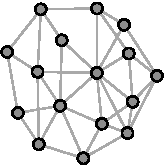
\includegraphics[width=.33\textwidth]{homophNet} & \hspace{2cm} &
	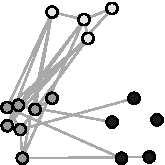
\includegraphics[width=.33\textwidth]{stochEquivNet}	
	\end{tabular}
	\caption{Graph on the left is a representation of an undirected network that exhibits a high degree of homophily, while on the right we show an undirected network that exhibits stochastic equivalence. }
	\label{fig:homphStochEquivNet}
\end{figure}

Another third-order dependence pattern that cannot be accounted for in the additive effects framework is stochastic equivalence. A pair of actors $ij$ are stochastically equivalent if the probability of $i$ relating to, and being related to, by every other actor is the same as the probability for $j$. This refers to the idea that there will be groups of nodes in a network with similar relational patterns. The occurrence of a dependence pattern such as this is not uncommon in the social science applications. \citet{manger:etal:2012} posit and estimate a stochastic equivalence structure to explain the formation of preferential trade agreements (PTAs). 
Specifically, they suggest that PTA formation is related to differences in per capita income levels between countries. Countries falling into high, middle, and low income per capita levels will have patterns of PTA formation that are determined by the groups into which they fall. %They find that PTA formation occurs with greater probability in the following-order high-middle, high-high, and middle-middle income groups, and that low income countries are rather unlikely to form PTAs with any partner.
Such a structure is represented in the right-most panel of Figure~\ref{fig:homphStochEquivNet}, here the lightly shaded group of nodes at the top can represent high-income countries, nodes on the bottom-left middle-income, and the darkest shade of nodes low-income countries. The behavior of actors in a network can at times be governed by group level dynamics, and failing to account for such dynamics leaves potentially important parts of the data generating process ignored. 

If we are able to explicitly model the variety of shared attributes that might cause third-order dependence patterns to develop, then the additive effects framework of the SRRM is likely enough to justify the conditional independence assumption that is central to the GLM framework. %The \pkg{amen} package provides for the estimation of the SRRM using a Bayesian framework. The main function in the \pkg{amen} package is titled ``ame'' and by default it runs a model assuming that no multiplicative effects are necessary. There is also a set of tools one can use to determine whether the inclusion of multiplicative effects is necessary.\footnote{We review these in the application section. Further discussion on how to use the \pkg{amen} package with examples can be found in \citet{hoff:2015:arxiv}.}
In the context of most observational research, however, the assumption that we have included all relevant explanatory variables is untenable. The implausibility of this assumption is, in spirit, the same reason why we no longer model time-series cross-sectional data without accounting for the temporal structure of the data.

\subsubsection{\textbf{Latent Variable Models}}

To account for third-order dependence patterns within the context of the SRRM we turn to latent variable models, which have become a popular approach for modeling relational data in fields as diverse as biology to computer science to the social sciences. These models assumes that relationships between nodes are mediated by a small number ($K$) of node-specific unobserved latent variables. One reason for their increased usage is that they enable researchers to capture and visualize third-order dependencies in a way that other approaches are not able to replicate. Additionally, the conditional independence assumption eliminates the model degeneracy issue, facilitates the testing of a variety of nodal and dyadic level theories, and provides a range of computational advantages \citep{hunter:etal:2012}. 

A number of major latent variable approaches have been developed to represent third-order dependencies in relational data, we focus on two here: the latent distance model and the latent factor model.\footnote{Though latent distance models have become a popular modeling tool in some disciplines \citep{salter:etal:2012}, we are aware of only one publication that has used this approach in political science, see \citet{kirkland:2012}. The bi-linear latent space approach, however, has been used in a variety of works in political science.} For the sake of exposition, we consider the case where relations are symmetric to describe the differences between these approaches. Both of these approaches can be incorporated into an undirected version of the framework that we have been constructing through the inclusion of an additional term to the model for $y_{ij}$, $\alpha(u_{i}, u_{j})$, that captures latent third-order characteristics of a network, where $u_{i}$ and $u_{j}$ are node-specific latent variables. General definitions for how $\alpha(u_{i}, u_{j})$ is defined for these latent variable models are shown in Equations~\ref{eqn:latAlpha}. One other point of note about these approaches is that researchers have to specify a value for $K$. In the case of the latent distance and factor models, a value of $K$ equal to two or three is typically large enough to account for third-order dependencies in relational data. 
%In the next section, we will discuss a set of diagnostic that help researchers to make this choice.

\begin{align}
\begin{aligned}
% \text{Latent class model} \\
% 	&\alpha(u_{i}, u_{j}) = m_{u_{i}, u_{j}} \\
% 	&u_{i} \in \{1, \ldots, K \}, \; i \in \{1,\ldots, n\} \\
% 	&M \text{ a } K \times K \text{ symmetric matrix} \\
\text{Latent distance model} \\
	&\alpha(\textbf{u}_{i}, \textbf{u}_{j}) = -|\textbf{u}_{i} - \textbf{u}_{j}| \\
	&\textbf{u}_{i} \in \mathbb{R}^{K}, \; i \in \{1, \ldots, n \} \\
\text{Latent factor model} \\
	&\alpha(\textbf{u}_{i}, \textbf{u}_{j}) = \textbf{u}_{i}^{T} \Lambda \textbf{u}_{j} \\
	&\textbf{u}_{i} \in \mathbb{R}^{K}, \; i \in \{1, \ldots, n \} \\
	&\Lambda \text{ a } K \times K \text{ diagonal matrix}
\label{eqn:latAlpha}
\end{aligned}
\end{align}

% In the latent class model (aka stochastic block model) each node $i$ is a member of some unknown latent class, $u_{i} \in (1,\ldots,K)$, and a probability distribution is used to describe the relationships among classes  \citep{nowicki:snijders:2001}. The probability of a tie between $i$ and $j$ is purely a function of the classes to which they belong. Nodes in a common class are stochastically equivalent, meaning if $i$ and $j$ are in the same class that the probability distribution for the relations that $i$ has is the same as the distribution for relations that $j$ has. Given that the probability of a tie between a pair of actors is wholely dependent upon the class to which they belong, nodes in the same class may have small or high probability of ties. A graph such as the one depicted in the left panel of Figure~\ref{fig:homphStochEquivNet} cannot be represented adequately through this type of approach. To do so, would require a large number of classes, $K$, that would not be particularly cohesive or distinguishable from one another.%\footnote{At the same time it is important to note that the characteristics of the latent class model make it ideal for other inferential goals such as community detection.}

The latent distance model was developed by \citet{hoff:etal:2002} to capture homophily. In this approach, each node $i$ has some unknown latent position in $K$ dimensional space, $\textbf{u}_{i} \in \mathbb{R}^{K}$, and the probability of a tie between a pair $ij$ is a function of the negative Euclidean distance between them: $-|\textbf{u}_{i} - \textbf{u}_{j}|$. \citet{hoff:etal:2002} show that because latent distances for a triple of actors obey the triangle inequality, this formulation models the tendencies toward homophily commonly found in social networks. This approach has been operationalized in the \pkg{latentnet} package developed by \citet{krivitsky:handcock:2015}. However, this approach also comes with an important shortcoming: it confounds stochastic equivalence and homophily. Consider two nodes $i$ and $j$ that are proximate to one another in $K$ dimensional Euclidean space, this suggests not only that $|\textbf{u}_{i} - \textbf{u}_{j}|$ is small but also that $|\textbf{u}_{i} - \textbf{u}_{l}| \approx |\textbf{u}_{j} - \textbf{u}_{l}|$, the result being that nodes $i$ and $j$ will by construction assumed to possess the same relational patterns with other actors such as $l$ (i.e., that they are stochastically equivalent).%\footnote{\citet{hoff:2008} shows that the only way to account for a network that exhibits stochastic equivalence through a latent distance model is by setting the number of latent dimensions, $K$, to be on the-order of the class membership size.}
Thus latent distance models confound strong ties with stochastic equivalence. This approach cannot adequately model data with many ties between nodes that have different network roles. 

An early iteration of the latent factor approach was presented in \citet{hoff:2005} and introduced to political science by \citet{hoff:ward:2004}, but the revised approach is motivated by an eigenvalue decomposition of a network.\footnote{An important difference in the earlier approaches such as the GBME compared to the model that we present here is that $\Lambda$ was taken to be the identity matrix thus stochastic equivalence could not be characterized. This approach should also not be confused with the projection model introduced in \citet{hoff:etal:2002}.} The motivation for this alternative framework stems from the fact that many real networks exhibit varying degrees of stochastic equivalence and homophily. In these situations, using either the latent distance or class model would end up representing only a part of the network structure. In the latent factor model, each actor has an unobserved vector of characteristics, $\textbf{u}_{i} = \{u_{i,1}, \ldots, u_{i,K} \}$, which describe their behavior as an actor in the network. The probability of a tie from $i$ to $j$ depends on the extent to which $\textbf{u}_{i}$ and $\textbf{u}_{j}$ are ``similar'' (i.e., point in the same direction) and on whether the entries of $\Lambda$ are greater than or less than zero. 

More specifically, the similarity in the latent factors, $\textbf{u}_{i} \approx \textbf{u}_{j}$, corresponds to how stochastically equivalent a pair of actors are and the eigenvalue determines whether the network exhibits positive or negative homophily. For example, say that that we estimate a rank-one latent factor model (i.e., $K=1$), in this case $\textbf{u}_{i}$ is represented by a scalar $u_{i,1}$, similarly, $\textbf{u}_{j}=u_{j,1}$, and $\Lambda$ will have just one diagonal element $\lambda$. The average effect this will have on $y_{ij}$ is simply $\lambda \times u_{i} \times u_{j}$, where a positive value of $\lambda>0$ indicates homophily and $\lambda<0$ anti-homophily. \citet{hoff:2008} shows that such a model can represent both homophily and stochastic equivalence, and that the alternative latent variable approaches can be represented as a latent factor model but not vice versa. In the directed version of this approach, we use the singular value decomposition,\footnote{The singular value decomposition is a model based analogue to the eigenvalue decomposition for directed networks.} here actors in the network have a vector of latent characteristics to describe their behavior as a sender, denoted by $\textbf{u}$, and as a receiver, $\textbf{v}$: $\textbf{u}_{i}, \textbf{v}_{j} \in \mathbb{R}^{K}$ \citep{hoff:2009}. These again can alter the probability, or in the continuous case value, of an interaction between $ij$ additively: $\textbf{u}_{i}^{T} \textbf{D} \textbf{v}_{j}$, where $\textbf{D}$ is an $n \times n$ diagonal matrix. 
The latent factor model is incorporated into the AME approach as a multiplicative effect to account for third-order dependencies \citep{hoff:2009,hoff:etal:2015}.  

Merging either of these approaches into the additive effects probit framework is possible through the addition of a term that captures third-order interdependencies. In the \pkg{latentnet} package this is done by directly incorporating $|\textbf{u}_{i} - \textbf{u}_{j}|$ as a fixed effect: $\theta_{ij} = \bm\beta^{T} \mathbf{X}_{ij} - |\textbf{u}_{i} - \textbf{u}_{j}|$.\footnote{The \pkg{latentnet} package also allows for the specification of a bilinear latent space that is closely related to the projection model introduced in \citet{hoff:etal:2002}.} However, incorporating the term in this way can affect our estimation of the linear relationship between the exogenous nodal and dyadic covariates. This results from collinearity between that set of exogenous attributes and the nodal positions of actors in the latent space. The intuition behind why collinearity occurs is not surprising given our discussion above. The latent space is essentially used to capture dependencies that can result from shared attributes between nodes. Thus if a particular exogenous covariate is actually predictive of relations between $i$ and $j$, due to homophily, this effect will be correlated with the nodal positions of actors in a $K$ dimensional Euclidean space. Additionally, interpretation of exogenous covariates is not as straightforward because the coefficients will be modeling a ``max value'' between nodes, if nodes had the same latent position. In the latent factor framework, this is not an issue because each of the random effect terms used to account for interdependencies has a mean of zero. The parameter estimates for the exogenous covariates from the latent factor approach can be interpreted as the average effect they have on the dependent variable after having accounted for network dependencies. The AME approach considers the regression model shown in Equation~\ref{eqn:ame}:

\begin{align}
\begin{aligned}
	y_{ij} &= g(\theta_{ij}) \\ 
	&\theta_{ij} = \bm\beta^{T} \mathbf{X}_{ij} + e_{ij} \\
	&e_{ij} = a_{i} + b_{j}  + \epsilon_{ij} + \alpha(\textbf{u}_{i}, \textbf{v}_{j}) \text{  , where } \\
	&\qquad \alpha(\textbf{u}_{i}, \textbf{v}_{j}) = \textbf{u}_{i}^{T} \textbf{D} \textbf{v}_{j} = \sum_{k \in K} d_{k} u_{ik} v_{jk} \\ 
\label{eqn:ame}
\end{aligned}
\end{align}

Using this framework, we are able to model the dyadic observations as conditionally independent given $\bm\theta$, where $\bm\theta$ depends on the the unobserved random effects, $\mathbf{e}$. $\mathbf{e}$ is then modeled to account for the potential first, second, and third-order dependencies that we have discussed. As described in Equation~\ref{eqn:srmCov}, $a_{i} + b_{j}  + \epsilon_{ij}$, are the additive random effects in this framework and account for sender, receiver, and within-dyad dependence. The multiplicative effects, $\textbf{u}_{i}^{T} \textbf{D} \textbf{v}_{j}$, are used to capture higher-order dependence patterns that are left over in $\bm\theta$ after accounting for any known covariate information. Thus the third-order interdependencies captured in the latent factor space of AME are those that could not have been explained by the exogenous nodal and dyadic covariates that have already been included in the model, or the additive row and column random effects. A Bayesian procedure in which parameters are iteratively updated using a Gibbs sampler is available in the \pkg{amen} package to estimate this type of generalized linear mixed effects model from continuous, binary, ordinal, and other relational data types.\footnote{The set of parameters that are estimated in the model from the observed data, $\{\mathbf{Y}, \mathbf{X}\}$, are: latent Gaussian variables ($\bm\theta$); nodal and/or dyadic regression coefficients ($\bm\beta$); additive nodal random effects ($\{(a_{i},b_{i})\} \in \{i=1, \ldots, n \}$); network covariance ($\Sigma_{ab},\, \Sigma_{\epsilon}$); multiplicative effects ($\mathbf{U}$, $\mathbf{V}$, and $\mathbf{D}$). Further details on this process can be found in \citet{hoff:2005} and \citet{hoff:2009}.}

Taken together, the additive effects portion of AME (described by the SRM) and the multiplicative effects (described by the latent factor model) provide a modeling framework similar to the GLMs that many scholars currently use, and has the benefit of being able to not only deal with interdependencies in relational data but also provide explicit estimates of these dependencies after having taken into account observable information. Specifically, we can obtain degree based effects for actors in the network, the level of reciprocity between actors, and also visualize the third-order interdependencies that remain in the data. This latter point is important to note as effectively using these visualizations may also help users of this approach to determine whether or not the inclusion of some other dyadic or nodal variable is necessary to accounting for patterns such as homophily or stochastic equivalence. 

\subsubsection{\textbf{ERGMs}}

An alternative approach to accounting for third-order dependence patterns are ERGMs. %This approach was first developed by \citet{erdos:renyi:1959}, and has became more widely understood as it has been applied to particular problems. \citet{frank:1971} undertook an early examination and Julian Besag developed interesting applications and methods promoting their examination \citep{besag:1977b}. But obtaining estimates was computational challenging and it was not until \citet{frank:strauss:1986} and \citet{wasserman:pattison:1996} that these methods found widespread application.
ERGM approaches are useful when researchers are interested in the role that a specific list of network statistics have in giving rise to a certain network. These network statistics could include the number of transitive triads in a network, balanced triads, reciprocal pairs and so on.\footnote{\citet{snijders:etal:2006} provides a detailed list of network statistics that can be included in an ERGM model specification.} In the ERGM framework, a set of statistics, $S(\mathbf{Y})$, define a model. Given the chosen set of statistics, the probability of observing a particular network dataset $\mathbf{Y}$ can be expressed as:

\begin{align}
\Pr(Y = y) = \frac{ \exp( \bm\beta^{T} S(y)  )  }{ \sum_{z \in \mathcal{Y}} \exp( \bm\beta^{T} S(z)  )  } \text{ ,  } y \in \mathcal{Y}
\label{eqn:ergm}
\end{align}

$\bm\beta$ represents a vector of model coefficients for the specified network statistics, $\mathcal{Y}$ denotes the set of all obtainable networks, and the denominator is used as a normalizing factor \citep{hunter:etal:2008}. This approach provides a way to state that the probability of observing a given network depends on the patterns that it exhibits, which are operationalized in the list of network statistics specified by the researcher. Within this approach one can test the role that a variety of network statistics play in giving rise to a particular network. %Further because of the Hammersley-Clifford theorem any probability distribution over networks can be represented by the form shown in Equation~\ref{eqn:ergm} \citep{hammersley:clifford:1971}. 

One issue that arises when conducting statistical inference with this model is in the calculation of the normalizing factor, which is what ensures that the expression above corresponds to a legitimate probability distribution. For even a trivially sized directed network that has only $20$ actors, calculating the denominator means summing over $2^{20\times(20-1)} = 2^{380}$ possible networks, or, to put it another way, more than the total number of atoms in the universe. One of the first approaches to deal with this issue was a computationally fast pseudo-likelihood approach developed by \citet{strauss:ikeda:1990}. However, this approach ignores the interdependent nature of observations in relational data, as a result, many have argued that the standard errors remain unreliable \citep{vanduijn:etal:2009}. %Additionally, there is no asymptotic theory underlying this approach on which to base the construction of confidence intervals and hypothesis tests \citep{kolaczyk:2009}.
The pseudo-likelihood approach has became increasingly unpopular in recent years among those in the network analysis community, particularly, as simulation based techniques have developed--though it has not disappeared. One favored approach in the literature is to approximate the MLE using Markov Chain Monte Carlo techniques, also referred to as MCMC-MLE.
% \citep{geyer:thompson:1992,snijders:2002,handcock:2003b}. 
%MCMC-MLE is based on a stochastic approximation of the log-likelihood and a maximization of the approximation; the \pkg{ergm} $\sf{R}$ package developed by \citet{hunter:etal:2008} provides for the estimation of this type of model.

\nocite{hammersley:clifford:1971}
The MCMC-MLE approach is an advancement but notable problems remain. \citet{chatterjee:diaconis:2013} have shown that MCMC procedures can take an exponential time to converge for broad classes of ERGMs unless the dyadic observations are independent. This is a result of the fact that MCMC procedures visit an infinitesimally small portion of the set of possible graphs. A related issue when estimating ERGMs is that the estimated model can become degenerate even if the observed graph is not degenerate. This means that the model is placing a large amount of probability on a small subset of networks that fall in the set of obtainable networks, $\mathcal{Y}$, but share little resemblance with the observed network \citep{schweinberger:2011}.
%\footnote{For example, most of the probability may be placed on empty graphs, no edges between nodes, or nearly complete graphs, almost every node is connected by an edge.} 
Some have argued that model degeneracy is simply a result of model misspecification \citep{goodreau:etal:2008,handcock:etal:2008}. This points to an important caveat in interpreting the implications of an often cited basis for ERGM, the Hammersley-Clifford theorem. Though this theorem ensures that any network can be represented through an ERGM, it says nothing about the complexity of the sufficient statistics ($S(y)$) required to do so. Failure to properly account for higher-order dependence structures through an appropriate specification can at best lead to model degeneracy, which provides an obvious indication that the specification needs to be altered, and at worst deliver a result that converges but does not appropriately capture the interdependencies in the network. The consequence of the latter case is a set of inferences that will continue to be biased as a result of unmeasured heterogeneity, thus defeating the major motivation for pursuing an inferential network model in the first place.%\footnote{A recent handbook on using network approaches to research political issues is found in \citet{victor:etal:2016}.  Recent research that uses exponential random graph models includes \citet{victor:ringe:2009}, \citet{berardo:scholz:2010}, \citet{calvo:leiras:2012}, \citet{lubell:etal:2012},   \citet{aleman:calvo:2013}, \citet{heaney:2014}, and \citet{kirkland:williams:2014}.}

In the following section we undertake a comparison of the latent distance model, ERGM, and the AME model using an application chosen by \citet{cranmer:etal:2016}.%\footnote{We disregard the latent class model here as it is primarily used as a community detection tool.}
In doing so, we are able to highlight the benefits that the AME model provides over alternatives.


\section{\textbf{Empirical Comparison}} 

%We utilize the same network dataset found in \citet{cranmer:etal:2016}.

\citet[p. 8]{cranmer:etal:2016} note that scholars must model third-order effects and ``must also specify them in a complete and correct manner'' or the ERGM model will be misspecified. To avoid providing an incorrect specification when comparing ERGM, we use the specification that they stipulated as theoretically correct. Their application utilizes a cross-sectional network measuring whether an actor indicated that they collaborated with another during the policy design of the Swiss CO$_{2}$ act \citep{ingold:2008}.\footnote{This is a directed relational matrix as an actor $i$ can indicate that they collaborated with $j$ but $j$ may not have stated that they collaborated with $i$.} The Swiss government proposed this act in 1995 with the goal of undertaking a 10\% reduction in CO$_{2}$ emissions by 2012. The act was accepted in the Swiss Parliament in 2000 and implemented in 2008. \citet{ingold:2008}, and subsequent work by \citet{ingold:fischer:2014}, sought to determine what drives collaboration among actors trying to affect climate change policy. The set of actors included in this network are those that were identified by experts as holding an important position in Swiss climate policy.\footnote{For further details on the methodology utilized in choosing the set of actors see \citet{ingold:2008,ingold:fischer:2014}.} In total, \citet{ingold:2008} identifies 34 relevant actors: five state actors, eleven industry and business representatives, seven environmental NGOs and civil society organizations, five political parties, and six scientific institutions and consultants. 

\begin{figure}[ht]
	\centering
	\begin{tabular}{cc}
	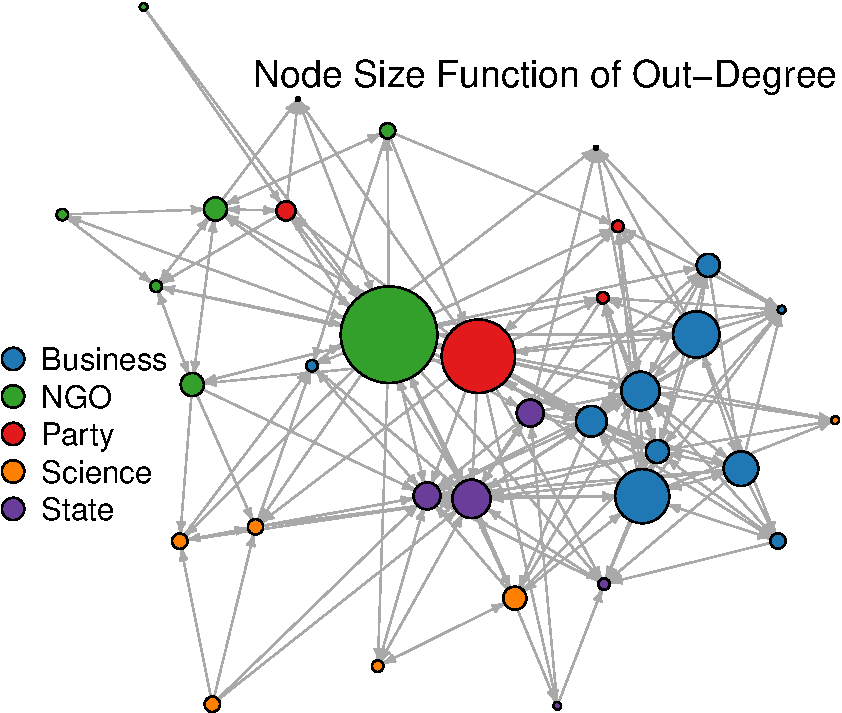
\includegraphics[width=.47\textwidth]{dvNet_outDegree} & 
	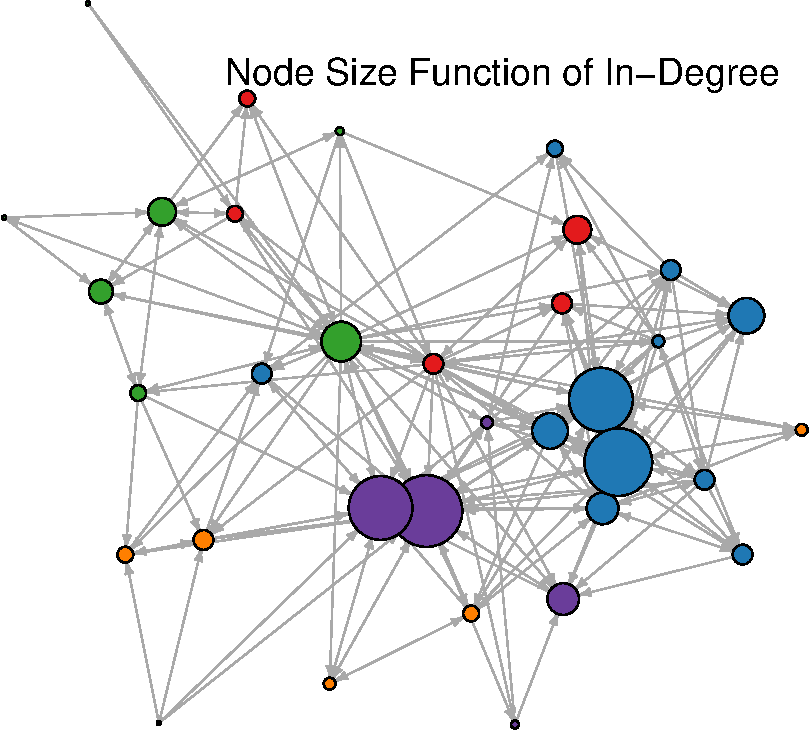
\includegraphics[width=.44\textwidth]{dvNet_inDegree}
	\end{tabular}
	\caption{Network visualizations of the Swiss climate change mitigation network. Nodes are colored by type of actor, and directed edges indicate relationships between actors. The network on the left weights node size by the number of out-going ties, and on the right the number of incoming-ties.}
	\label{fig:dvNet}
\end{figure}
\FloatBarrier

Figure~\ref{fig:dvNet} provides visualizations for this directed collaboration network. Nodes are colored by the type of actor and a directed edge indicates an actor stated that they collaborated with another, and determining which actor indicated the collaboration can be ascertained by the direction of the arrow. 
%Actor positions are estimated using a force-directed layout algorithm.\footnote{To determine the positions of nodes in this network we use the Fruchterman-Reingold algorithm \citep{fruchterman:reingold:1991}. These types of algorithms use information contained within the structure of the network itself to construct depictions of graphs. A straightforward way to understand how they work is to think of nodes connected by edges as particles that are attracted to each other, and nodes that are unconnected as particles that repulse each other. These types of algorithms simulate a system in which nodes pull and push upon each other until they reach an equilibrium position.} 
The majority of industry and business actors are clustering together, meaning that these types of actors tend to indicate they collaborated with one another during the policy design process. Three of the state actors are pushed towards the center of the graph because they share relationships with many actors in the network. Most of the actors classified as scientific institutions are pushed towards the far left border of the graphs as it seems they tend to interact among themselves and just a few of the other actors. 

%An important part of our discussion from the previous section revolved around the idea that within network structures we find variation in how active nodes are in engaging with others in the network. 
To illustrate nodal heterogeneity in the case of the Swiss climate change mitigation networks we weight the size of nodes, in the network on the left, by the number of their outgoing ties, and on the right by their incoming ties. From the network on the left, we can see that each of the scientific institutions and consultants shown in Figure~\ref{fig:dvNet} indicate that they collaborate with relatively few organizations, especially, in comparison with actors from industry and business. Additionally, there is even variation within actor types as evidenced by differences amongst NGO or political party actors. Similar findings of nodal heterogeneity emerge if we turn our attention to examining nodes by their incoming ties. 

%Collaboration among these 34 actors is not simply a function of actor type.
To understand what factors may play a role in shaping collaboration in this relational data structure a modeling approach is necessary. \citet{cranmer:etal:2016} follow \citet{ingold:fischer:2014} in developing a model specification. We do not review the specification in detail here, instead we just provide a summary of the variables to be included and the theoretical expectations of their effects in Table~\ref{tab:theorySpec}. 

% \newcolumntype{L}{>{\arraybackslash}m{9cm}}
% \begin{table}[ht]
% \centering
% \begingroup\scriptsize
% \begin{tabular}{lLc}
% \footnotesize{\textbf{Variable}} & \footnotesize{\textbf{Description}} & \footnotesize{\textbf{Expected Effect}} \\ \hline\hline
% 	\multicolumn{3}{l}{\textbf{Conflicting policy preferences}} \\
% 	\quad Business v. NGO & Binary, dyadic covariate that equals one when one actor is from the business sector and the other an NGO. & $-$ \\
% 	\quad Opposition/alliance & Binary, dyadic covariate that equals one when $i$, sender, perceives $j$, receiver, as having similar policy objectives regarding climate change.  & $+$ \\
% 	\quad Preference dissimilarity & Transformation of four core beliefs into a Manhattan distance matrix, smaller the distance the closer the beliefs of $i$ and $j$. & $-$ \\
% 	\multicolumn{3}{l}{\textbf{Transaction costs}} \\
% 	\quad Joint forum participation & Binary, dyadic covariate that equals one when $i$ and $j$ belong to the same policy forum. & $+$ \\
% 	\multicolumn{3}{l}{\textbf{Influence}} \\
% 	\quad Influence attribution & Binary, dyadic covariate that equals one when $i$ considers $j$ to be influential. & $+$ \\
% 	\quad Alter's influence in-degree & Number of actors that mention $i$ as being influential, this is a measure of reputational power. & $+$ \\
% 	\quad Influence absolute diff. & Absolute difference in reputational power between $i$ and $j$. & $-$ \\
% 	\quad Alter = Government Actor & Binary, nodal covariate that equals one when $j$ is a state actor. & $+$ \\
% 	\multicolumn{3}{l}{\textbf{Functional requirements}} \\
% 	\quad Ego = Environment NGO & Binary, nodal covariate that equals one when $i$ is an NGO. & $+$ \\
% 	\quad Same actor type & Binary, dyadic covariate that equals when $i$ and $j$ are the same actor type. & $+$ \\
% 	\multicolumn{3}{l}{\textbf{Endogenous dependencies: ERGM Specific Parameters}} \\
% 	\quad Mutuality & Captures concept of reciprocity, if $i$ indicates they collaborated with $j$ then $j$ likely collaborates with $i$. & $+$\\
% 	\quad Outdegree popularity & Captures idea that actors sending more ties will be more popular targets themselves for collaboration.  & $+$ \\
% 	\quad Twopaths & Counts the number of two-paths in the network, two-path is an instance where $i$ is connected to $j$, $j$ to $k$, but $i$ is not connected to $k$. & $-$ \\
% 	\quad GWIdegree (2.0) & Takes into account how many ties a node sends in the network, used to capture network structures that result from some highly active nodes.  & $+$ \\
% 	\quad GWESP (1.0) & Counts the number of shared partners for each pair and sums across.  & $+$ \\
% 	\quad GWOdegree (0.5) & Takes into account how many ties a node receives in the network, used to capture networks structures that result from some highly popular nodes.  & $+$ \\
% \hline\hline
% \end{tabular}
% \endgroup
% \caption{Summary of variables to be included in model specification. With the exception of mutuality, each of the parameters falling in the Endogenous dependencies grouping are only explicitly testable through ERGM. }
% \label{tab:theorySpec}
% \end{table}
% \FloatBarrier

\subsection{Parameter Estimates}

Using the specification described in Table~\ref{tab:theorySpec} we compare five different modeling approaches. The first four approaches chosen here, as in \citet{cranmer:etal:2016}, are a logistic regression model, MRQAP, ERGM, and a latent space model (LSM) in which third-order dependencies are accounted for via a two-dimensional Euclidean distance metric.\footnote{For a detailed discussion on the MRQAP see \citet{dekker:etal:2007}.} Parameter estimates for these four approaches are shown in Table~\ref{tab:regTable}. 

The fifth column shows the results from using the additive and multiplicative effects model (AME), in which we account for nodal and dyadic heterogeneity using the SRM and third-order effects represented by a latent factor approach in which we set $K=2$.\footnote{Table~\ref{tab:regTable_ame} in Section~\ref{sec:ameVsAmeAppendix} of the Appendix shows that the parameter estimates presented here for the AME model remain very similar no matter the $K$ chosen.} \citet{cranmer:etal:2016} provide a lengthy discussion of the differences between the first four modelling approaches that we will not repeat here. More relevant for us are how parameter estimates from AME relate to other approaches. The first point to note is that, in general, the parameter estimates returned by the AME are similar to those of MRQAP and ERGM but quite different from the LSM. For example, while the LSM returns a result for the \texttt{Opposition/alliance} variable that diverges from MRQAP and ERGM, the AME returns a result that is not only similar to those approaches but in line with the theoretical expectations of \citet{ingold:fischer:2014}. Similar discrepancies between LSM and other approaches appear for parameters such as \texttt{Influence attribution} and \texttt{Alter's influence degree}. Each of these discrepancies are resolved when using AME. In part, this is a function of  how the LSM approach as operationalized in the \pkg{latentnet} package can confound the effects of covariates with the latent space metric.\footnote{As shown in Table~\ref{tab:regTable_latSpace} in Section~\ref{sec:ameVsLatentnetAppendix} of the Appendix, these differences persist even when incorporating sender and receiver random effects or when switching to a bilinear approach to handle third-order dependencies.} % Additionally, the coefficients from the LSM are modeling a ``max value'' between nodes, if nodes had the same latent position. 

% latex table generated in R 3.3.1 by xtable 1.8-2 package
% Sun Aug 21 03:32:43 2016
\begin{table}[ht]
\centering
\begingroup\normalsize
\begin{tabular}{lccccc}
   & Logit & MRQAP & LSM & ERGM & AME \\ 
  \hline
\hline
Intercept/Edges & -4.44$^{\ast}$ & -4.24$^{\ast}$ & 0.94$^{\ast}$ & -12.17$^{\ast}$ & -3.39$^{\ast}$ \\ 
   & (0.34) &  & [0.09; 1.82] & (1.40) & [-4.38; -2.50] \\ 
  \textbf{Conflicting policy preferences} &  &  &  &  &  \\ 
  $\;\;\;\;$ Business vs. NGO & -0.86 & -0.87$^{\ast}$ & -1.37$^{\ast}$ & -1.11$^{\ast}$ & -1.37$^{\ast}$ \\ 
   & (0.46) &  & [-2.42; -0.41] & (0.51) & [-2.44; -0.47] \\ 
  $\;\;\;\;$ Opposition/alliance & 1.21$^{\ast}$ & 1.14$^{\ast}$ & 0.00 & 1.22$^{\ast}$ & 1.08$^{\ast}$ \\ 
   & (0.20) &  & [-0.40; 0.39] & (0.20) & [0.72; 1.47] \\ 
  $\;\;\;\;$ Preference dissimilarity & -0.07 & -0.60 & -1.76$^{\ast}$ & -0.44 & -0.79$^{\ast}$ \\ 
   & (0.37) &  & [-2.62; -0.90] & (0.39) & [-1.55; -0.08] \\ 
  \textbf{Transaction costs} &  &  &  &  &  \\ 
  $\;\;\;\;$ Joint forum participation & 0.88$^{\ast}$ & 0.75$^{\ast}$ & 1.51$^{\ast}$ & 0.90$^{\ast}$ & 0.92$^{\ast}$ \\ 
   & (0.27) &  & [0.86; 2.17] & (0.28) & [0.40; 1.47] \\ 
  \textbf{Influence} &  &  &  &  &  \\ 
  $\;\;\;\;$ Influence attribution & 1.20$^{\ast}$ & 1.29$^{\ast}$ & 0.08 & 1.00$^{\ast}$ & 1.09$^{\ast}$ \\ 
   & (0.22) &  & [-0.40; 0.55] & (0.21) & [0.69; 1.53] \\ 
  $\;\;\;\;$ Alter's influence indegree & 0.10$^{\ast}$ & 0.11$^{\ast}$ & 0.01 & 0.21$^{\ast}$ & 0.11$^{\ast}$ \\ 
   & (0.02) &  & [-0.03; 0.04] & (0.04) & [0.07; 0.15] \\ 
  $\;\;\;\;$ Influence absolute diff. & -0.03$^{\ast}$ & -0.06$^{\ast}$ & 0.04 & -0.05$^{\ast}$ & -0.07$^{\ast}$ \\ 
   & (0.02) &  & [-0.01; 0.09] & (0.01) & [-0.11; -0.03] \\ 
  $\;\;\;\;$ Alter = Government actor & 0.63$^{\ast}$ & 0.68 & -0.46 & 1.04$^{\ast}$ & 0.55 \\ 
   & (0.25) &  & [-1.08; 0.14] & (0.34) & [-0.07; 1.15] \\ 
  \textbf{Functional requirements} &  &  &  &  &  \\ 
  $\;\;\;\;$ Ego = Environmental NGO & 0.88$^{\ast}$ & 0.99 & -0.60 & 0.79$^{\ast}$ & 0.67 \\ 
   & (0.26) &  & [-1.32; 0.09] & (0.17) & [-0.38; 1.71] \\ 
  $\;\;\;\;$ Same actor type & 0.74$^{\ast}$ & 1.12$^{\ast}$ & 1.17$^{\ast}$ & 0.99$^{\ast}$ & 1.04$^{\ast}$ \\ 
   & (0.22) &  & [0.63; 1.71] & (0.23) & [0.63; 1.50] \\ 
  \textbf{Endogenous dependencies} &  &  &  &  &  \\ 
  $\;\;\;\;$ Mutuality & 1.22$^{\ast}$ & 1.00$^{\ast}$ &  & 0.81$^{\ast}$ & 0.39 \\ 
   & (0.21) &  &  & (0.25) & [-0.12; 0.96] \\ 
  $\;\;\;\;$ Outdegree popularity &  &  &  & 0.95$^{\ast}$ &  \\ 
   &  &  &  & (0.09) &  \\ 
  $\;\;\;\;$ Twopaths &  &  &  & -0.04$^{\ast}$ &  \\ 
   &  &  &  & (0.02) &  \\ 
  $\;\;\;\;$ GWIdegree (2.0) &  &  &  & 3.42$^{\ast}$ &  \\ 
   &  &  &  & (1.47) &  \\ 
  $\;\;\;\;$ GWESP (1.0) &  &  &  & 0.58$^{\ast}$ &  \\ 
   &  &  &  & (0.16) &  \\ 
  $\;\;\;\;$ GWOdegree (0.5) &  &  &  & 8.42$^{\ast}$ &  \\ 
   &  &  &  & (2.11) &  \\ 
   \hline
\hline
\end{tabular}
\endgroup
\caption{* p $<$ 0.05. Logistic regression and ERGM results are shown with standard errors in parentheses. MRQAP provides no standard errors. LSM and AME are shown with 95\% posterior credible intervals provided in brackets.} 
\label{tab:regTable}
\end{table}

\FloatBarrier

There are also notable differences between the parameter estimates that result from the MRQAP, ERGM, and the AME. Using the AME we find evidence that \texttt{Preference dissimilarity} is associated with a reduced probability of collaboration between a pair of actors, which is in line with the theoretical expectations stated earlier. Additionally, the AME and MRQAP results differ from ERGM for the nodal effects related to whether a receiver of a collaboration is a government actor, \texttt{Alter=Government actor}, and whether the sender is an environmental NGO, \texttt{Ego=Environmental NGO}.

When it comes to estimating higher-order effects, ERGM is able to provide explicit estimates of a variety of higher-order parameters, however, this comes with the caveat that these are the ``right'' set of endogenous dependencies. The AME approach, as shown in Equation~\ref{eqn:ame}, estimates network dependencies by examining patterns left over after taking into account the observed covariates. For the sake of space, we focus on examining the third-order dependencies left over after accounting for the observed covariates and network covariance structure modeled by the SRM. A visualization of remaining third-order dependencies is shown in Figure~\ref{fig:uv}. 

\begin{figure}[ht]
\centering
	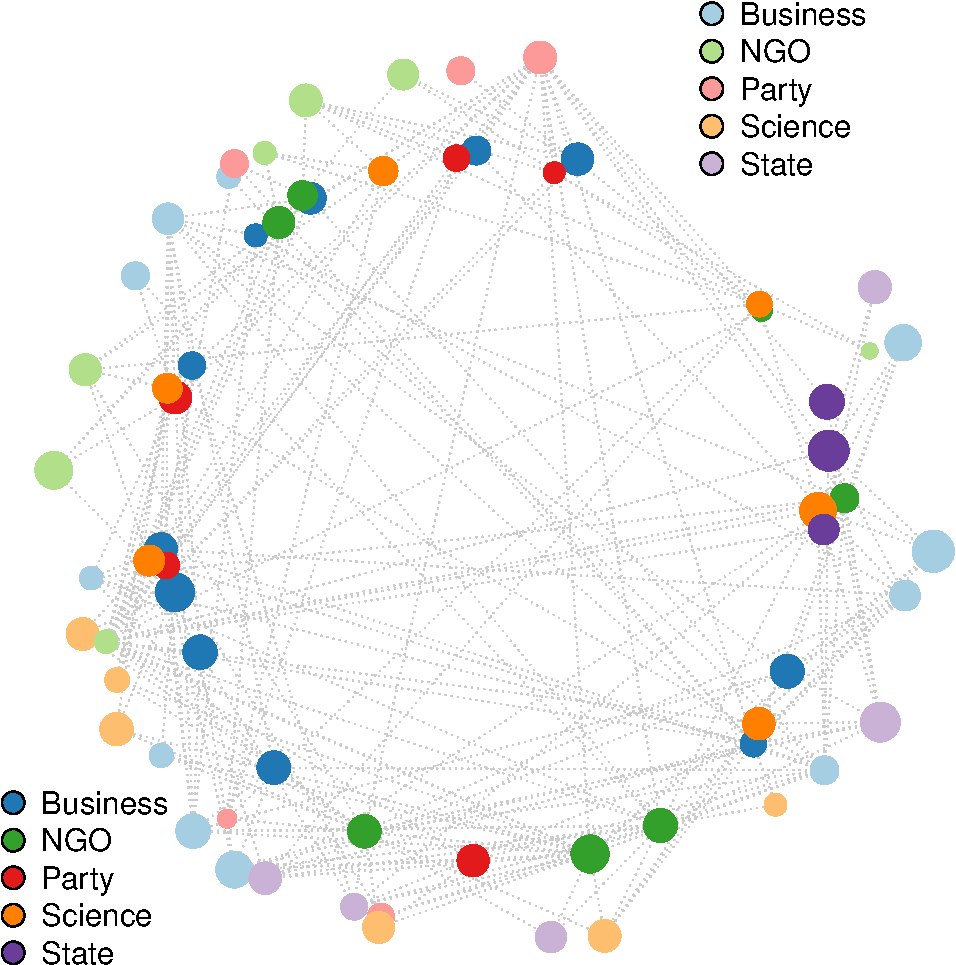
\includegraphics[width=.5\textwidth]{ameFitSR_2_UV}
	\caption{Circle plot of estimated latent factors.}
	\label{fig:uv}
\end{figure}
\FloatBarrier

In Figure~\ref{fig:uv}, the directions of $\hat{u}_{i}$'s and $\hat{v}_{i}$'s are noted in lighter and darker shades, respectively, of an actor's type.\footnote{For example, actors from industry and business are assigned a color of blue and the direction of $\hat{u}_{i}$ for these actors is shown in light blue and $\hat{v}_{i}$ in dark blue} The size of actors is a function of the magnitude of the vectors, and dashed lines between actors indicate greater than expected levels of collaboration based on the regression term and additive effects. In the case of the application dataset that we are using here organization names have been anonymized and no additional covariate information is available. However, if we were to observe nodes sharing certain attributes clustering together in this circle plot that would mean such an attribute could be an important factor in helping us to understand collaborations among actors in this network. Given how actors of different types are distributed in almost a random fashion in this plot, we can at least be sure that it is unlikely other third-order patterns can be picked up by that factor.

\subsection{Tie Formation Prediction}

How do these approaches fit the data out-of-sample? We utilize a cross-validation procedure to assess the out-of-sample performance for each of the models presented in Table~\ref{tab:regTable} as follows:

\begin{itemize}
	\item Randomly divide the $n \times (n-1)$ data points into $S$ sets of roughly equal size, letting $s_{ij}$ be the set to which pair $\{ij\}$ is assigned.
	\item For each $s \in \{1, \ldots, S\}$:
	\begin{itemize}
		\item Obtain estimates of the model parameters conditional on $\{y_{ij} : s_{ij} \neq s\}$, the data on pairs not in set $s$.
		\item For pairs $\{kl\}$ in set $s$, let $\hat y_{kl} = E[y_{kl} | \{y_{ij} : s_{ij} \neq s\}]$, the predicted value of $y_{kl}$ obtained using data not in set $s$.
	\end{itemize}
\end{itemize}

The procedure summarized in the steps above generates a sociomatrix of out-of-sample predictions of the observed data. Each entry $\hat y_{ij}$ is a predicted value obtained from using a subset of the data that does not include $y_{ij}$. In this application we set $S$ to 45 which corresponds to randomly excluding approximately 2\% of the data from the estimation. Such a low number of observations were excluded in every fold because excluding any more observations would cause the ERGM specification to result in a degenerate model that empirically can not be fit. This highlights the computational difficulties associated with ERGMs in the presence of even small levels of missingness.  Not only do you have to have the exactly correct model specification, you also have to have virtually all of the data on the true network.

\begin{figure}[ht]
	\centering
	\begin{tabular}{cc}
	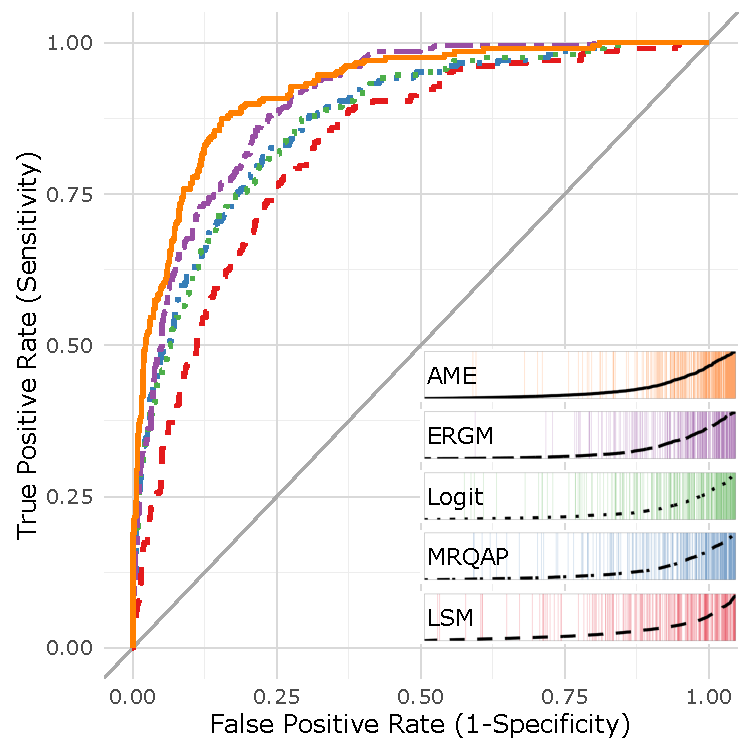
\includegraphics[width=.5\textwidth]{roc_outSample} & 
	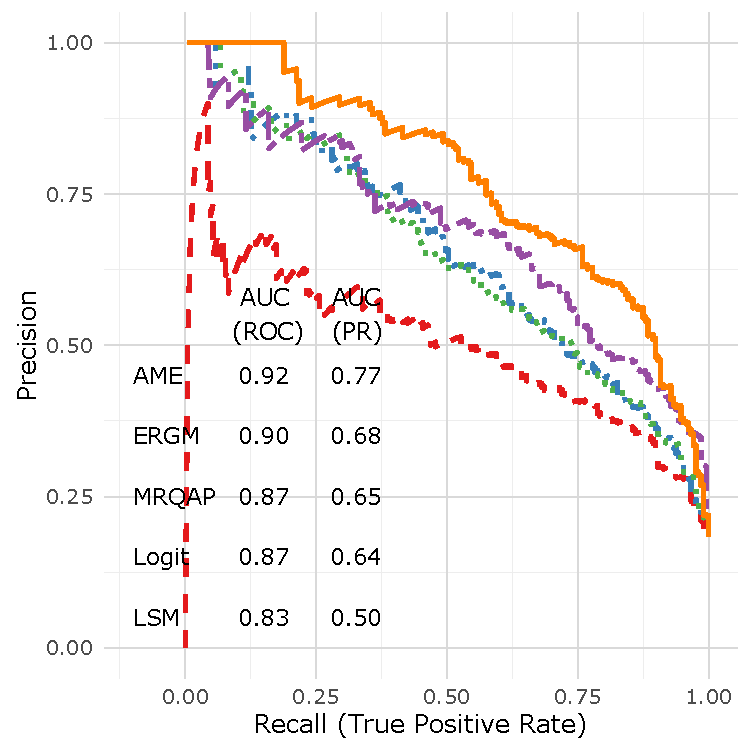
\includegraphics[width=.5\textwidth]{rocPr_outSample}	
	\end{tabular}
	\caption{Assessments of out-of-sample predictive performance using ROC curves, separation plots, and PR curves. AUC statistics are provided as well for both curves.}
	\label{fig:roc}
\end{figure}
\FloatBarrier

Using the set of out-of-sample predictions we generate from the cross-validation procedure, we provide a series of tests to assess model fit. First, is a diagnostic that is common in the political science literature. The left-most plot in Figure~\ref{fig:roc} compares the five approaches in terms of their ability to predict the out-of-sample occurrence of collaboration based on Receiver Operating Characteristic (ROC) curves. ROC curves provide a comparison of the trade-off between the True Positive Rate (TPR), sensitivity, False Positive Rate (FPR), 1-specificity, for each model. %Models that have a better fit according to this test should have curves that follow the left-hand border and then the top border of the ROC space.
On this diagnostic, the AME model performs best closely followed by ERGM. The MRQAP and Logit approaches perform similarly, and the LSM approach lags notably behind the other specifications.\footnote{Figure~\ref{fig:roc_latentSpace} in the Appendix provides additional comparisons between our AME approach and various parameterizations of the LSM, in each case we find that the AME approach provides far superior results in terms of out-of-sample predictive performance. However, the LSM approach does begin to perform notably better when incorporating sender and receiver random effects. We also compare performance when using varying values of K for the AME model, we find that increasing $K$ to 3 or 4 does not improve out-of-sample model fit. Results are shown in Figure~\ref{fig:roc_ame}. Typically setting $K=2$ works well for most applied cases.} 

A more intuitive visualization of the differences between these modeling approaches can be gleaned through examining the separation plots included on the right-bottom edge of the ROC plot. This visualization tool plots each of the observations, in this case actor pairs, in the dataset according to their predicted value from left (low values) to right (high values). Models with a good fit should have all network links, here these are colored by the modeling approach, towards the right of the plot. Using this type of visualization we can again see that the AME and ERGM models performs better than the alternatives.

The last diagnostic we highlight to assess predictive performance are precision-recall (PR) curves. In both ROC and PR space we utilize the TPR, also referred to as recall--though in the former it is plotted on the y-axis and the latter the x-axis. The difference, however, is that in ROC space we utilize the FPR, while in PR space we use precision. FPR measures the fraction of negative examples that are misclassified as positive, while precision measures the fraction of examples classified as positive that are truly positive. PR curves are useful in situations where correctly predicting events is more interesting than simply predicting non-events \citep{davis:goadrich:2006}. This is especially relevant in the context of studying many relational datasets in political science such as conflict, because events in such data are extremely sparse and it is relatively easy to correctly predict non-events. In the case of our application dataset, the vast majority of dyads, 80\%, do not have a network linkage, which points to the relevance of assessing performance using the PR curves as we do in the right-most plot of Figure~\ref{fig:roc}. We can see that the relative-ordering of the models remains similar but the differences in how well they perform become much more stark. Here we find that the AME approach performs notably better in actually predicting network linkages than each of the alternatives. Area under the curve (AUC) statistics are provided in Figure~\ref{fig:roc} and these also highlight AME's superior out-of-sample performance.

\subsection{Capturing Network Attributes}

For network data it is also important to assess whether a model adequately captures the network parameters of the dependent variable \citep{hunter:etal:2008}. To do this one can compare the observed network with a set of networks simulated from the estimated models. We restrict our focus to the three approaches--LSM, ERGM, and AME--that explicitly seek to model network interdependencies. We simulate 1,000 networks from the three models and compare how well they align with the observed network in terms of four network statistics: (1) the empirical standard deviation of the row means (i.e., heterogeneity of nodes in terms of the ties they send); (2) the empirical standard deviation of the column means (i.e., heterogeneity of nodes in terms of the ties they receive); (3) the empirical within-dyad correlation (i.e., measure of reciprocity in the network); and (4) a normalized measure of triadic dependence. A comparison of the LSM, ERGM, and AME models among these four statistics is shown in Figure~\ref{fig:ergmAmePerf}.\footnote{Scholars in the networks field usually test for more specific dependencies in order to ascertain whether a particular endogenous covariate needs to be added or modified. We perform this same performance exericise on a more specific set of statistics and visualize the results in Figure~\ref{gofAll} of the Appendix. There we also find that the AME does as well as ERGM, and that the LSM model lags behind.}

\begin{figure}[ht]
	\centering
	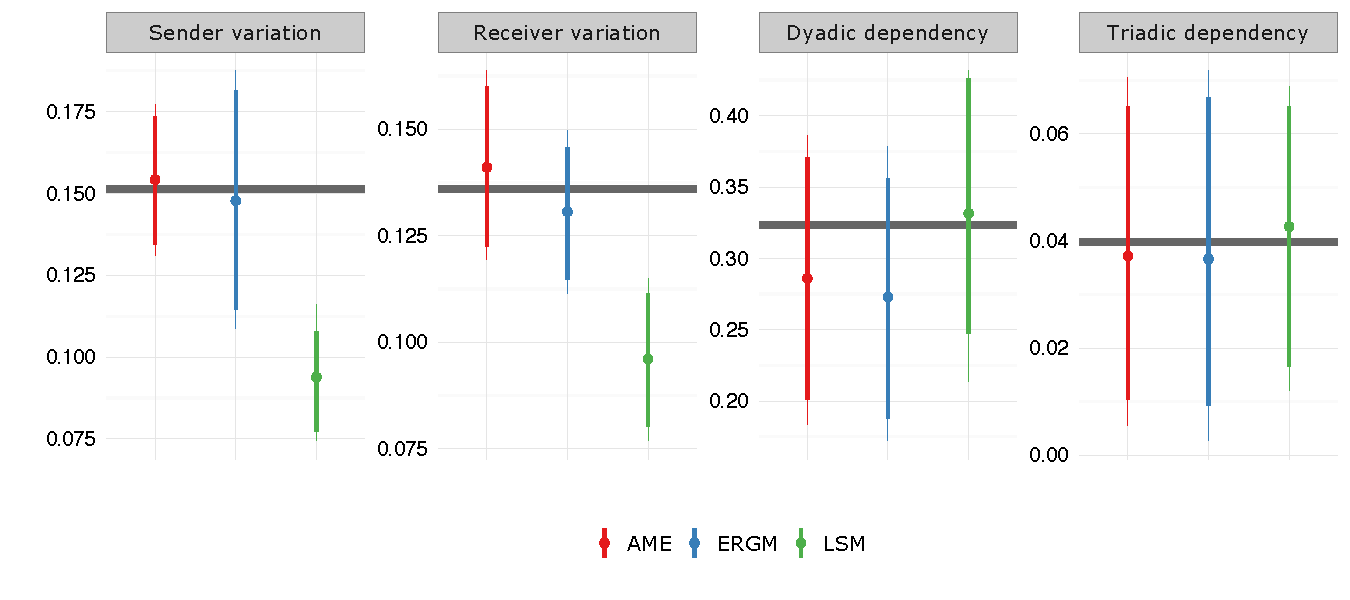
\includegraphics[width=1\textwidth]{netPerfCoef}
	\caption{Network goodness of fit summary using \pkg{amen}.}
	\label{fig:ergmAmePerf}
\end{figure}
\FloatBarrier

Here it becomes quickly apparent that the LSM model fails to capture how active and popular actors are in the Swiss climate change mitigation network.\footnote{Interestingly, even after incorporating random sender and receiver effects into the LSM framework this problem is not completely resolved, see Figure~\ref{fig:netPerfCoef_latSpace} in the Appendix for details.} The AME and ERGM specifications again both tend to do equally well.\footnote{Not surprisingly, if we increase $K$ in the AME approach we are able to better account for triadic dependencies, see Figure~\ref{fig:netPerfCoef_ameSR} in the Appendix for details.} If when running this diagnostic, we found that the AME model did not adequately represent the observed network this would indicate that we might want to increase $K$ to better account for network interdependencies. No changes to the model specification as described by the exogenous covariates a researcher has chosen would be necessary. If the ERGM results did not align with the diagnostic presented in Figure~\ref{fig:ergmAmePerf}, then this would indicate that an incorrect set of endogenous dependencies have been specified. Failing to identify (or find) the right specification will leave the researcher with the problems we introduced earlier.

\section{\textbf{Conclusion}}

The AME approach to estimation and inference in network data provides a number of benefits over alternative approaches. Specifically, it provides a modeling framework for dyadic data that is based on familiar statistical tools such as linear regression, GLM, random effects, and factor models. We have an understanding of how each of these tools work, they are numerically more stable than ERGM approaches, and more general than alternative latent variable models such as the latent distance or class frameworks. Further the estimation procedure utilized in AME avoids confounding the effects of nodal and dyadic covariates with actor positions in the latent space as the latent distance variable does. For researchers in international relations and more broadly across political science this is of primary interest, as many studies that employ relational data still have conceptualizations  that are monadic or dyadic in nature. Additionally, through the application dataset utilized herein we show that the AME approach outperforms both ERGM and latent distance models in out-of-sample prediction, and also is better able to capture network dependencies than the latent distance model. 

More broadly, relational data structures are composed of actors that are part of a system. It is unlikely that this system can be viewed simply as a collection of isolated actors or pairs of actors. The assumption  that dependencies between observations occur can at the very least be examined. Failure to take into account interdependencies leads to biased parameter estimates and poor fitting models. By using standard diagnostics such as shown in Figures~\ref{fig:gofAll} and \ref{fig:ergmAmePerf}, one can easily assess whether an assumption of independence is reasonable. We stress this point because a common misunderstanding that seems to have emerged within the political science literature relying on dyadic data is that a network based approach is only necessary if one has theoretical explanations that extend beyond the dyadic. This is not at all the case and findings that continue to employ a dyadic design may misrepresent the effects of the very variables that they are interested in. The AME approach that we have detailed here provides a statistically familiar way for scholars to account for unobserved network structures in relational data. Additionally, through this approach we can visualize these dependencies in order to better learn about the network patterns that remain in the event of interest after having accounted for observed covariates.  

When compared to other network based approaches such as ERGM, AME is easier to specify and utilize. It is also more straightforward to interpret since it does not require interpretation of unusual features such as \textit{three-stars} which fall outside of the normal language for discussing social science. Further, the \pkg{amen} package facilitates the modeling of longitudinal network data. In sum, excuses for continuing to treat relational data as conditionally independent are no longer valid. 

\clearpage

% \renewcommand{\thefigure}{A\arabic{figure}}
% \setcounter{figure}{0}
% \renewcommand{\thetable}{A.\arabic{table}}
% \setcounter{table}{0}
% \renewcommand{\thesection}{A.\arabic{section}}
% \setcounter{section}{0}

% \section{\textbf{Appendix}}

% \subsection{AME Model Convergence}
% \label{sec:ameConvAppendix}

% Trace plot for AME model presented in paper.  

% \begin{figure}[ht]
% 	\centering
% 	\begin{tabular}{cc}
% 	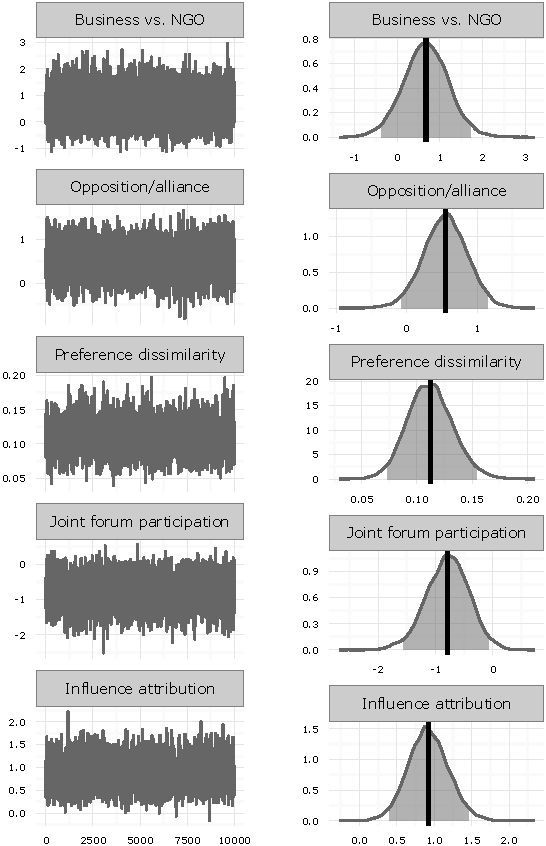
\includegraphics[width=.45\textwidth]{ameConv1_SR2} &
% 	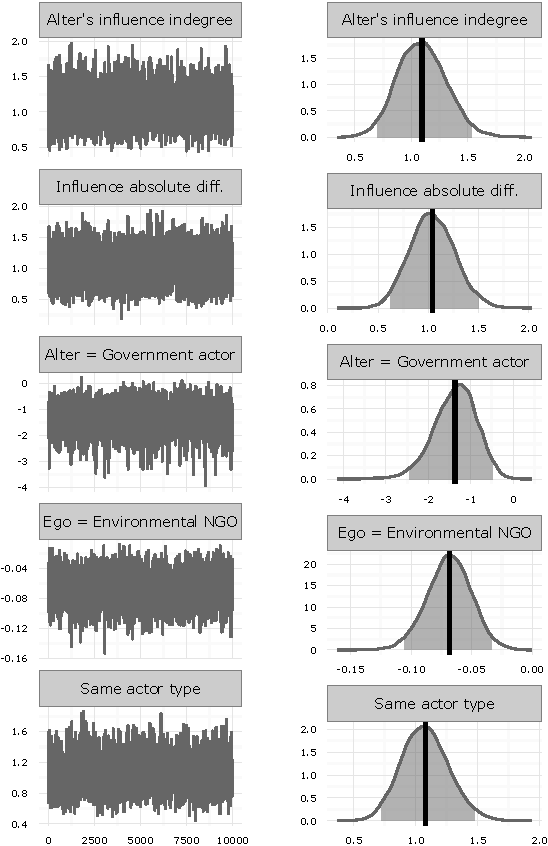
\includegraphics[width=.45\textwidth]{ameConv2_SR2}
% 	\end{tabular}
% 	\caption{Trace plot for AME model presented in paper. In this model, we utilize the SRM to account for first and second-order dependence. To account for third order dependencies we use the latent factor approach with $K=2$.}
% 	\label{fig:ameConv}
% \end{figure}
% \FloatBarrier
% \newpage

% \subsection{Other Network Goodness of Fit Tests}
% \label{sec:otherNetGof}
%
% Below we show a standard set of statistics upon which comparisons are usually conducted:\footnote{See \citet{morris:etal:2008} for details on each of these parameters. If one was to examine goodness of fit in the \pkg{ergm} package these parameters would be calculated by default.}
%
% \newcolumntype{L}{>{\arraybackslash}m{9cm}}
% \begin{table}[ht]
% \centering
% \begingroup\scriptsize
% \begin{tabular}{lL}
% \footnotesize{\textbf{Variable}} & \footnotesize{\textbf{Description}} \\ \hline\hline
% 	Dyad-wise shared partners & Number of dyads in the network with exactly $i$ shared partners. \\
% 	Edge-wise shared partners & Similar to above except this counts the number of dyads with the same number of edges. \\
% 	Geodesic distances & The proportion of pairs of nodes whose shortest connecting path is of length $k$, for $k=1,2,\ldots$. Also, pairs of nodes that are not connected are classified as $k=\infty$. \\
% 	Incoming k-star & Propensities for individuals to have connections with multiple network partners. \\
% 	Indegree & Proportion of nodes with the same value of the attribute as the receiving node. \\
% 	Outdegree & Proportion of nodes with the same value of the attribute as the sending node. \\
% \hline\hline
% \end{tabular}
% \endgroup
% \caption{Description of a set of standard statistics used to assess whether a model captures network dependencies. }
% \label{tab:netStat}
% \end{table}
% \FloatBarrier
%
% \begin{figure}[ht]
% 	\centering
% 	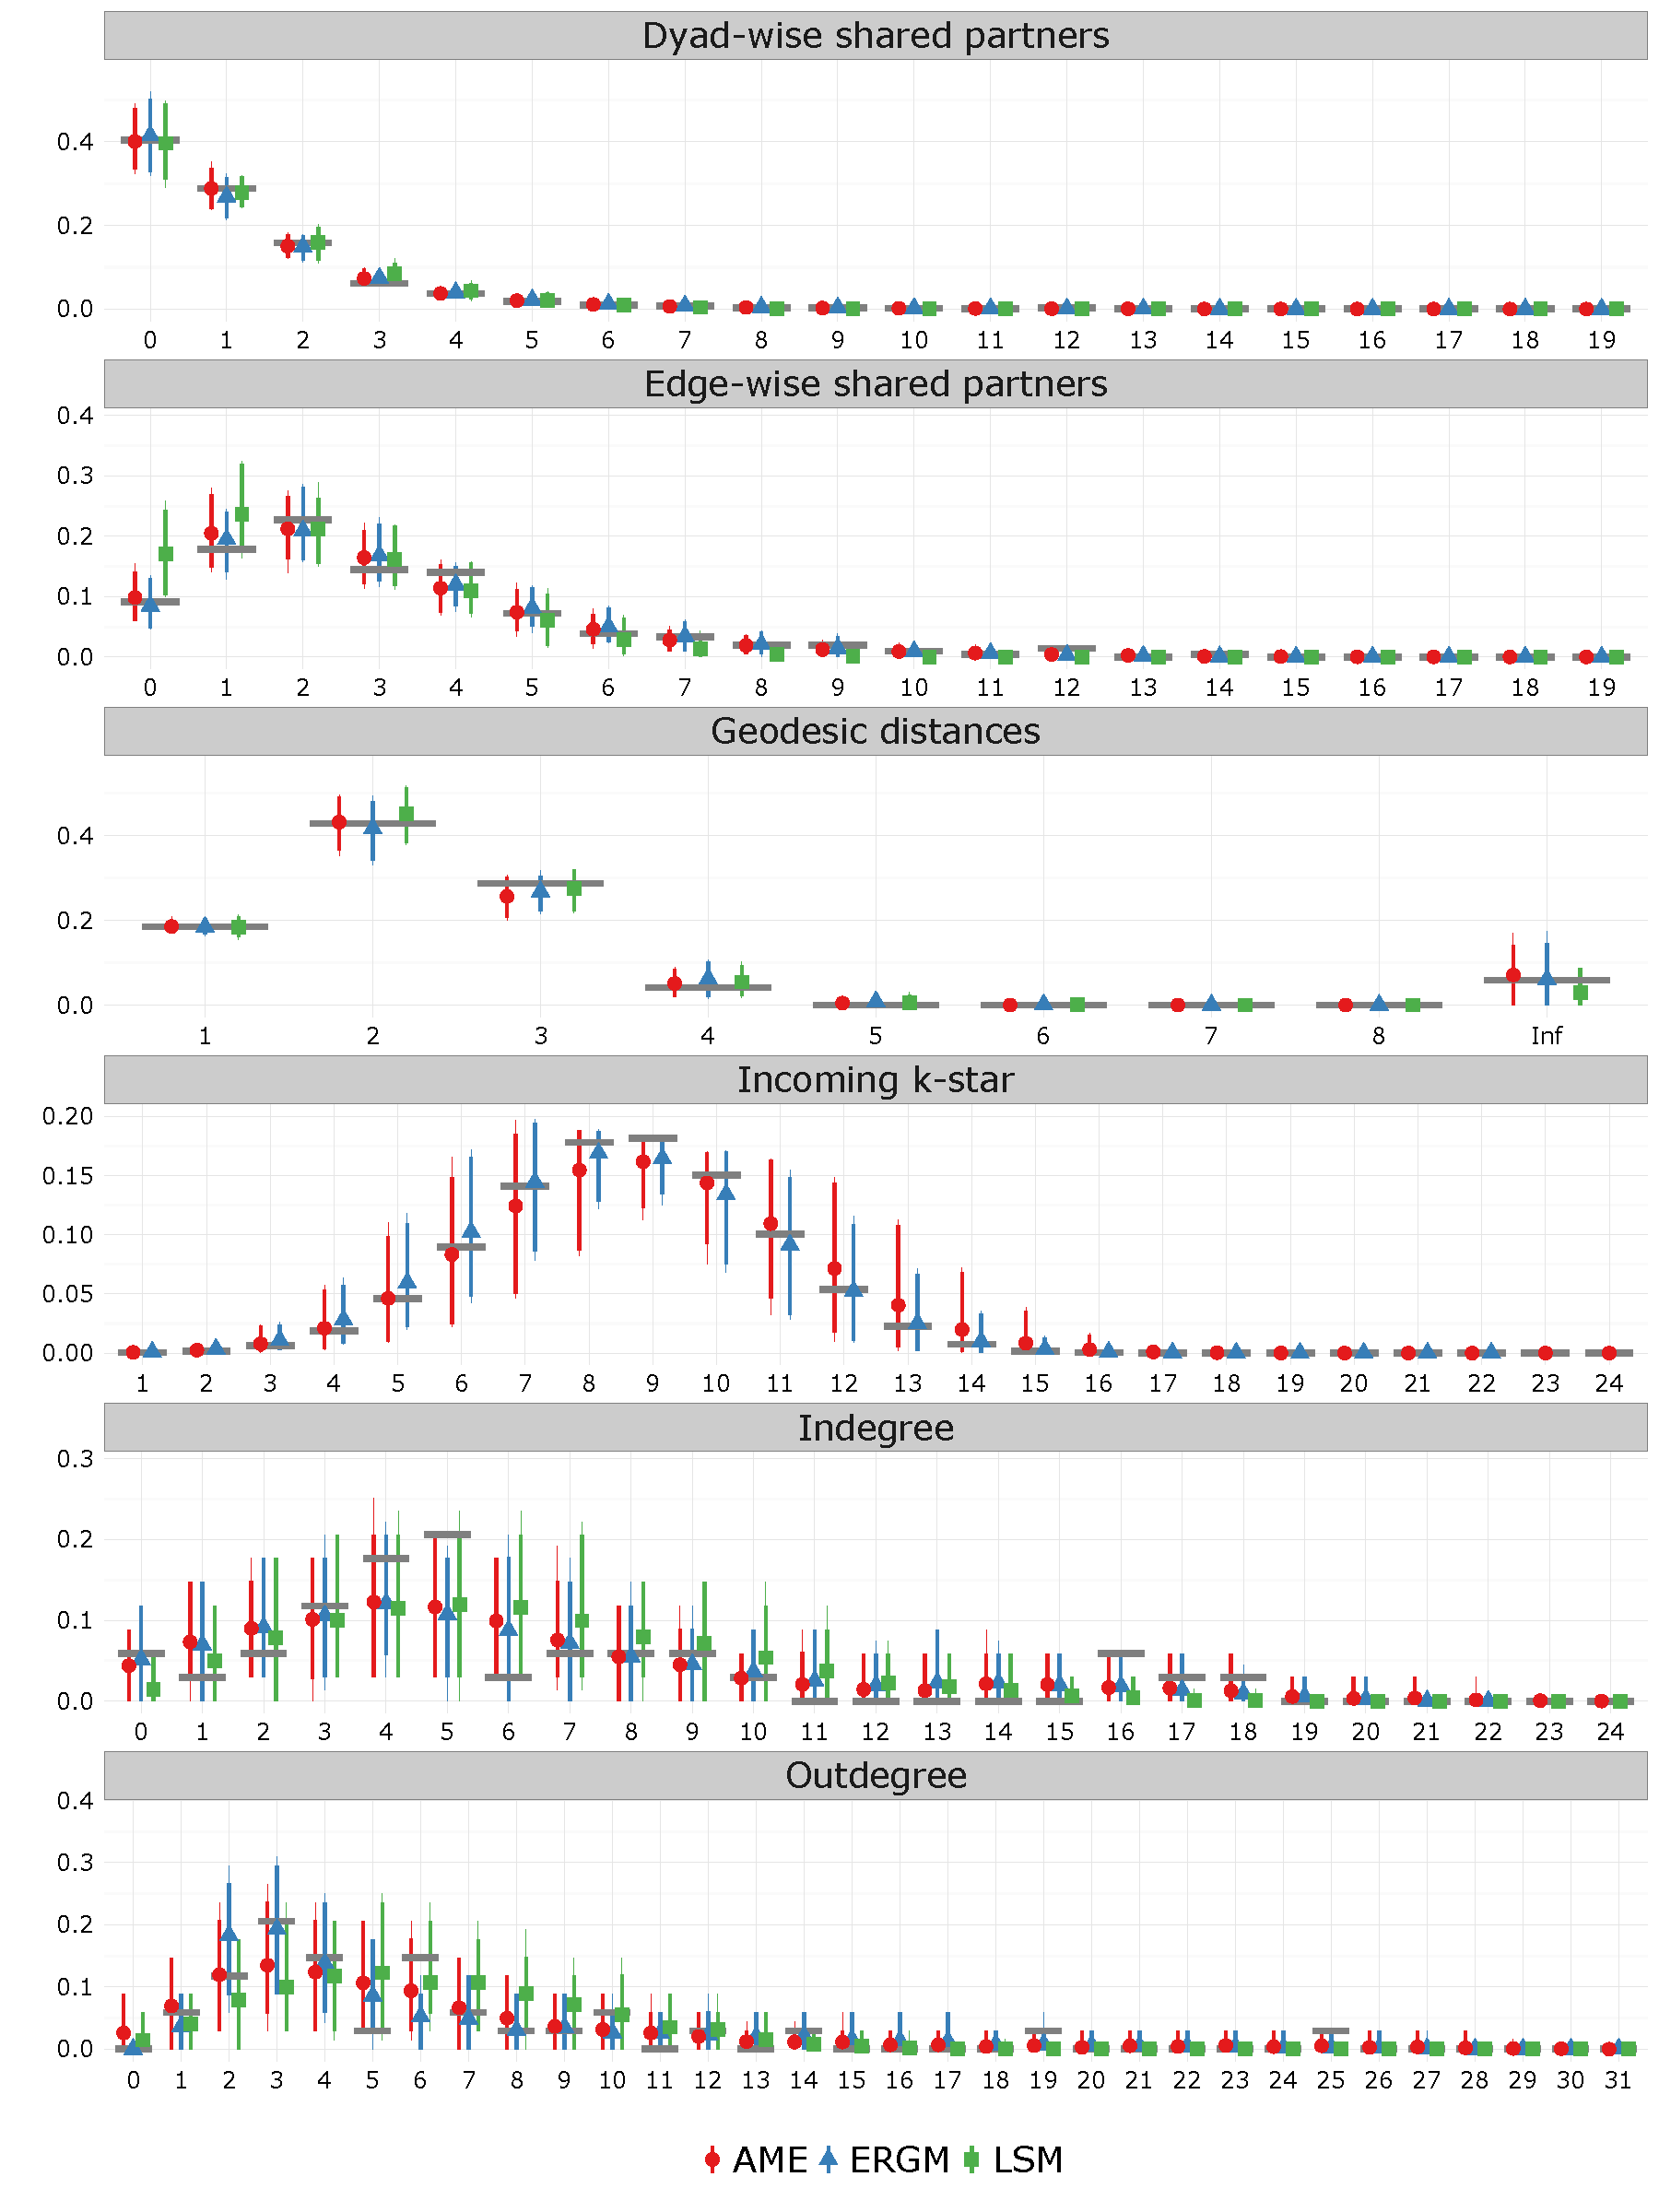
\includegraphics[width=1\textwidth]{ggGofAll}
% 	\caption{Goodness of fit statistics to assess how well the LSM, ERGM, and AME approaches account for network dependencies.}
% 	\label{fig:gofAll}
% \end{figure}
% \FloatBarrier
%
% We simulate 1,000 networks from the LSM, ERGM, and AME model and compare how well they align with the observed network in terms of the statistics described in Table~\ref{tab:netStat}. The results are shown in Figure~\ref{fig:gofAll}. Values for the observed network are indicated by a gray bar and average values from the simulated networks for the AME, ERGM, and LSM are represented by a diamond, triangle, and square, respectively. The densely shaded interval around each point represents the 95\% interval from the simulations and the taller, less dense the 90\% interval.\footnote{Calculation for the incoming k-star statistic is not currently supported by the \pkg{latentnet} package.} Looking across the panels in Figure~\ref{fig:gofAll} it is clear that there is little difference between the ERGM and AME models in terms of how well they capture network dependencies. The LSM model, however, does perform somewhat worse in comparison here as well. Particularly, when it comes to assessing the number of edge-wise shared partners and in terms of capturing the indegree and outdegree distributions of the collaboration network.

% \subsection{Comparison of \pkg{amen} \& \pkg{latentnet} $\sf{R}$ Packages}
% \label{sec:ameVsLatentnetAppendix}

% Here we provide a comparison of the AME model we present in the paper with a variety of parameterizations from the \pkg{latentnet} package. The number of dimensions in the latent space in each of these cases is set to 2. LSM (SR) represents a model in which random sender and receiver effects are included. LSM (Bilinear) represents a model in which a bilinear latent model term is used instead of the default Euclidean distance term. A bilinear latent model with sender and receiver random effects is not equivalent to the AME approach that we introduce here for reasons that we have already discussed in the paper. 

% % latex table generated in R 3.3.1 by xtable 1.8-2 package
% % Sun Aug 21 03:38:39 2016
% \begin{table}[ht]
% \centering
% \begingroup\tiny
% \begin{tabular}{lccccc}
%    & LSM & LSM (Bilinear) & LSM (SR) & LSM (Bilinear + SR) & AME \\ 
%   \hline
% \hline
% Intercept/Edges & 0.94$^{\ast}$ & -2.66$^{\ast}$ & 0.60 & -2.50$^{\ast}$ & -3.39$^{\ast}$ \\ 
%    & [0.09; 1.82] & [-3.53; -1.87] & [-1.10; 2.37] & [-4.14; -0.88] & [-4.38; -2.50] \\ 
%   \textbf{Conflicting policy preferences} &  &  &  &  &  \\ 
%   $\;\;\;\;$ Business vs. NGO & -1.37$^{\ast}$ & -2.64$^{\ast}$ & -3.07$^{\ast}$ & -2.87$^{\ast}$ & -1.37$^{\ast}$ \\ 
%    & [-2.42; -0.41] & [-4.61; -0.96] & [-4.77; -1.56] & [-4.63; -1.29] & [-2.44; -0.47] \\ 
%   $\;\;\;\;$ Opposition/alliance & 0.00 & 0.04 & 0.31 & 0.24 & 1.08$^{\ast}$ \\ 
%    & [-0.40; 0.39] & [-0.44; 0.54] & [-0.24; 0.86] & [-0.36; 0.82] & [0.72; 1.47] \\ 
%   $\;\;\;\;$ Preference dissimilarity & -1.76$^{\ast}$ & -2.00$^{\ast}$ & -1.88$^{\ast}$ & -2.20$^{\ast}$ & -0.79$^{\ast}$ \\ 
%    & [-2.62; -0.90] & [-3.01; -1.03] & [-3.07; -0.68] & [-3.46; -0.96] & [-1.55; -0.08] \\ 
%   \textbf{Transaction costs} &  &  &  &  &  \\ 
%   $\;\;\;\;$ Joint forum participation & 1.51$^{\ast}$ & 1.24$^{\ast}$ & 1.56$^{\ast}$ & 1.62$^{\ast}$ & 0.92$^{\ast}$ \\ 
%    & [0.86; 2.17] & [0.53; 1.93] & [0.69; 2.41] & [0.70; 2.52] & [0.40; 1.47] \\ 
%   \textbf{Influence} &  &  &  &  &  \\ 
%   $\;\;\;\;$ Influence attribution & 0.08 & -0.08 & 0.30 & 0.28 & 1.09$^{\ast}$ \\ 
%    & [-0.40; 0.55] & [-0.62; 0.46] & [-0.37; 0.96] & [-0.42; 0.97] & [0.69; 1.53] \\ 
%   $\;\;\;\;$ Alter's influence indegree & 0.01 & -0.05$^{\ast}$ & 0.06 & 0.05 & 0.11$^{\ast}$ \\ 
%    & [-0.03; 0.04] & [-0.09; -0.01] & [-0.03; 0.14] & [-0.04; 0.13] & [0.07; 0.15] \\ 
%   $\;\;\;\;$ Influence absolute diff. & 0.04 & 0.02 & -0.08$^{\ast}$ & -0.08$^{\ast}$ & -0.07$^{\ast}$ \\ 
%    & [-0.01; 0.09] & [-0.03; 0.07] & [-0.14; -0.02] & [-0.14; -0.02] & [-0.11; -0.03] \\ 
%   $\;\;\;\;$ Alter = Government actor & -0.46 & -0.80 & -0.11 & -0.20 & 0.55 \\ 
%    & [-1.08; 0.14] & [-1.67; 0.04] & [-1.91; 1.76] & [-2.14; 1.74] & [-0.07; 1.15] \\ 
%   \textbf{Functional requirements} &  &  &  &  &  \\ 
%   $\;\;\;\;$ Ego = Environmental NGO & -0.60 & -1.90$^{\ast}$ & -1.69 & -1.84 & 0.67 \\ 
%    & [-1.32; 0.09] & [-3.10; -0.86] & [-3.74; 0.23] & [-4.02; 0.11] & [-0.38; 1.71] \\ 
%   $\;\;\;\;$ Same actor type & 1.17$^{\ast}$ & 1.40$^{\ast}$ & 1.82$^{\ast}$ & 1.90$^{\ast}$ & 1.04$^{\ast}$ \\ 
%    & [0.63; 1.71] & [0.85; 1.95] & [1.10; 2.54] & [1.19; 2.62] & [0.63; 1.50] \\ 
%    \hline
% \hline
% \end{tabular}
% \endgroup
% \caption{* p $<$ 0.05. 95\% posterior credible intervals are provided in brackets.} 
% \label{tab:regTable_latSpace}
% \end{table}


% \begin{figure}[ht]
% 	\centering
% 	\begin{tabular}{cc}
% 	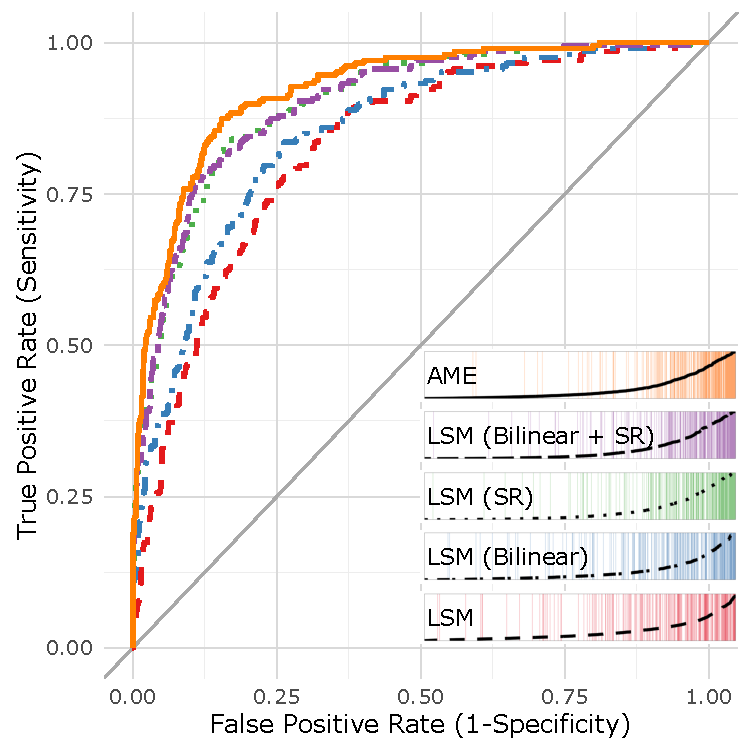
\includegraphics[width=.5\textwidth]{roc_latSpace_outSample} & 
% 	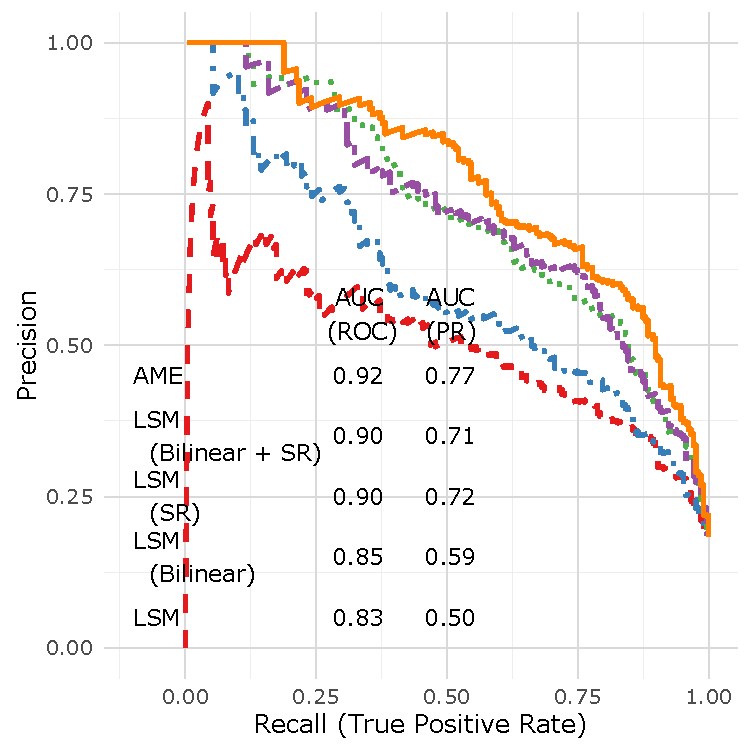
\includegraphics[width=.5\textwidth]{rocPr_latSpace_outSample}
% 	\end{tabular}
% 	\caption{Assessments of out-of-sample predictive performance using ROC curves, separation plots, and PR curves. AUC statistics are provided as well for both curves.}
% 	\label{fig:roc_latentSpace}
% \end{figure}

% \begin{figure}[ht]
% 	\centering
% 	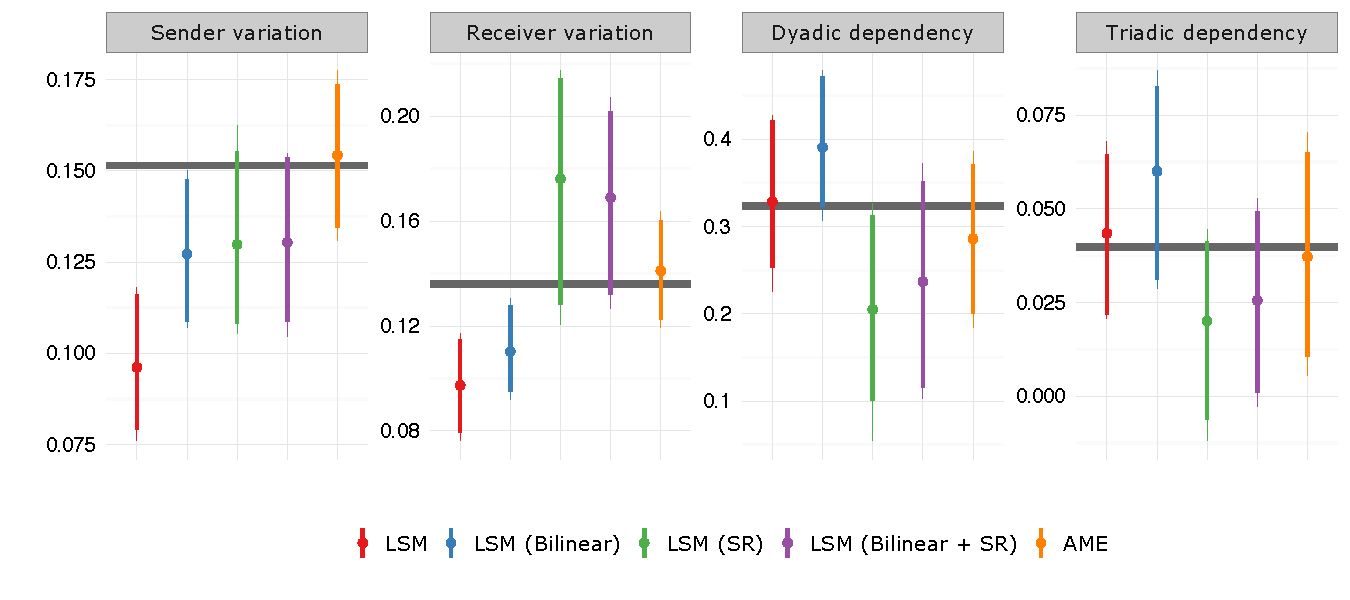
\includegraphics[width=1\textwidth]{netPerfCoef_latSpace}
% 	\caption{Network goodness of fit summary using \pkg{amen}.}
% 	\label{fig:netPerfCoef_latSpace}
% \end{figure}

% \FloatBarrier

% \clearpage
% \subsection{Comparison with other AME Parameterizations}
% \label{sec:ameVsAmeAppendix}

% Here we provide a comparison of the AME model we present in the paper that uses $K=2$ for multiplicative effects and show how results change when we use $K=\{1,3,4\}$. Trace plots for $K=\{1,3,4\}$ are available upon request.

% % latex table generated in R 3.3.1 by xtable 1.8-2 package
% % Tue Sep 27 12:34:36 2016
% \begin{table}[ht]
% \centering
% \begingroup\tiny
% \begin{tabular}{lcccc}
%    & AME (k=1) & AME (k=2) & AME (k=3) & AME (k=4) \\ 
%   \hline
% \hline
% Intercept/Edges & -3.08$^{\ast}$ & -3.39$^{\ast}$ & -3.72$^{\ast}$ & -3.93$^{\ast}$ \\ 
%    & [-3.91; -2.30] & [-4.38; -2.50] & [-4.84; -2.73] & [-5.12; -2.87] \\ 
%   \textbf{Conflicting policy preferences} &  &  &  &  \\ 
%   $\;\;\;\;$ Business vs. NGO & -1.28$^{\ast}$ & -1.37$^{\ast}$ & -1.48$^{\ast}$ & -1.51$^{\ast}$ \\ 
%    & [-2.20; -0.47] & [-2.44; -0.47] & [-2.63; -0.49] & [-2.69; -0.47] \\ 
%   $\;\;\;\;$ Opposition/alliance & 0.95$^{\ast}$ & 1.08$^{\ast}$ & 1.19$^{\ast}$ & 1.28$^{\ast}$ \\ 
%    & [0.64; 1.27] & [0.72; 1.47] & [0.80; 1.64] & [0.86; 1.77] \\ 
%   $\;\;\;\;$ Preference dissimilarity & -0.65$^{\ast}$ & -0.79$^{\ast}$ & -0.89$^{\ast}$ & -0.95$^{\ast}$ \\ 
%    & [-1.30; -0.03] & [-1.55; -0.08] & [-1.71; -0.12] & [-1.80; -0.14] \\ 
%   \textbf{Transaction costs} &  &  &  &  \\ 
%   $\;\;\;\;$ Joint forum participation & 0.84$^{\ast}$ & 0.92$^{\ast}$ & 1.01$^{\ast}$ & 1.06$^{\ast}$ \\ 
%    & [0.38; 1.31] & [0.40; 1.47] & [0.44; 1.62] & [0.43; 1.72] \\ 
%   \textbf{Influence} &  &  &  &  \\ 
%   $\;\;\;\;$ Influence attribution & 1.00$^{\ast}$ & 1.09$^{\ast}$ & 1.21$^{\ast}$ & 1.28$^{\ast}$ \\ 
%    & [0.63; 1.39] & [0.69; 1.53] & [0.75; 1.71] & [0.80; 1.84] \\ 
%   $\;\;\;\;$ Alter's influence indegree & 0.10$^{\ast}$ & 0.11$^{\ast}$ & 0.12$^{\ast}$ & 0.13$^{\ast}$ \\ 
%    & [0.07; 0.14] & [0.07; 0.15] & [0.08; 0.17] & [0.09; 0.18] \\ 
%   $\;\;\;\;$ Influence absolute diff. & -0.06$^{\ast}$ & -0.07$^{\ast}$ & -0.07$^{\ast}$ & -0.08$^{\ast}$ \\ 
%    & [-0.10; -0.03] & [-0.11; -0.03] & [-0.12; -0.04] & [-0.12; -0.04] \\ 
%   $\;\;\;\;$ Alter = Government actor & 0.52 & 0.55 & 0.60 & 0.64 \\ 
%    & [-0.04; 1.07] & [-0.07; 1.15] & [-0.07; 1.27] & [-0.07; 1.35] \\ 
%   \textbf{Functional requirements} &  &  &  &  \\ 
%   $\;\;\;\;$ Ego = Environmental NGO & 0.61 & 0.67 & 0.76 & 0.80 \\ 
%    & [-0.31; 1.56] & [-0.38; 1.71] & [-0.38; 1.90] & [-0.40; 2.04] \\ 
%   $\;\;\;\;$ Same actor type & 0.97$^{\ast}$ & 1.04$^{\ast}$ & 1.11$^{\ast}$ & 1.17$^{\ast}$ \\ 
%    & [0.60; 1.35] & [0.63; 1.50] & [0.64; 1.59] & [0.68; 1.68] \\ 
%    \hline
% \hline
% \end{tabular}
% \endgroup
% \caption{* p $<$ 0.05. 95\% posterior credible intervals are provided in brackets.} 
% \label{tab:regTable_ame}
% \end{table}


% \begin{figure}[ht]
% 	\centering
% 	\begin{tabular}{cc}
% 	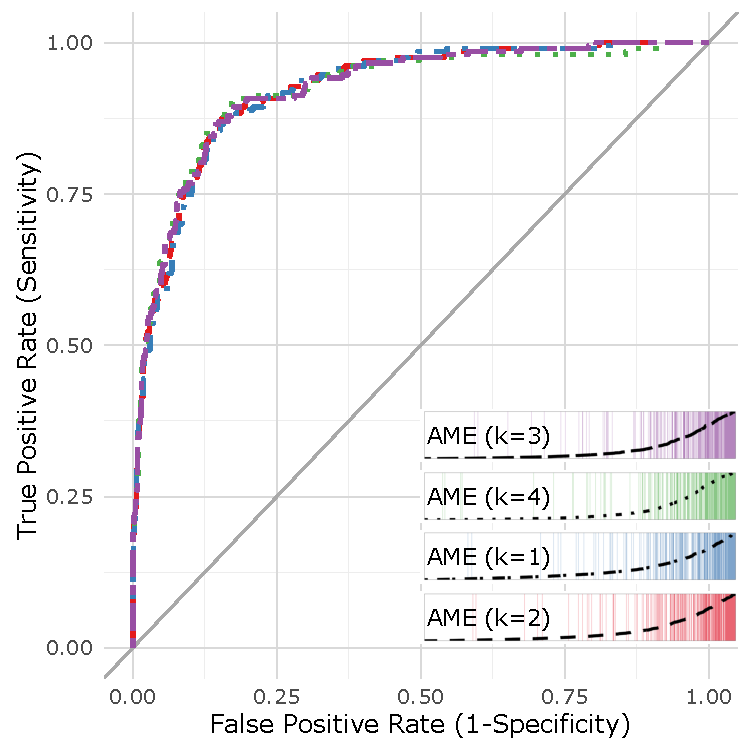
\includegraphics[width=.5\textwidth]{roc_ameSR_outSample} & 
% 	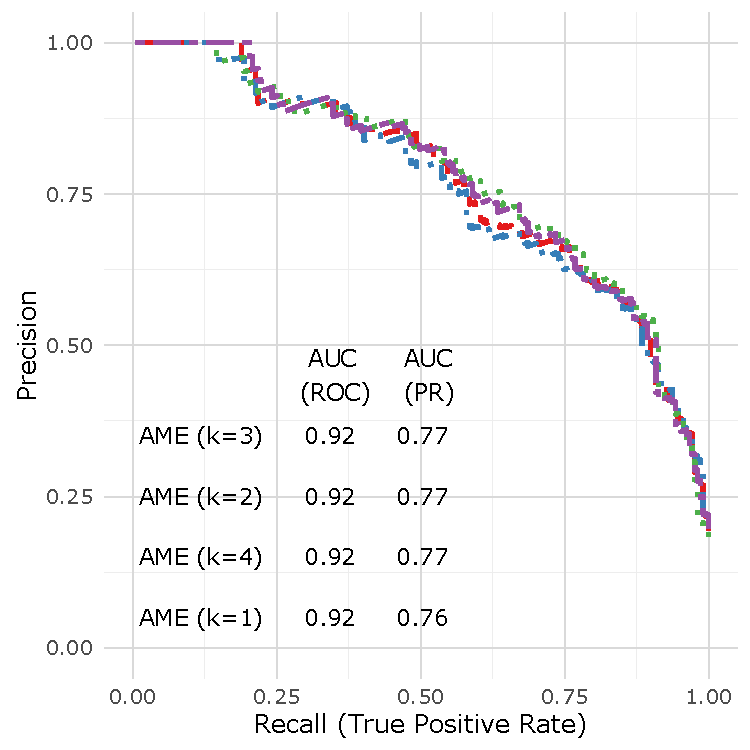
\includegraphics[width=.5\textwidth]{rocPr_ameSR_outSample}
% 	\end{tabular}
% 	\caption{Assessments of out-of-sample predictive performance using ROC curves, separation plots, and PR curves. AUC statistics are provided as well for both curves.}
% 	\label{fig:roc_ame}
% \end{figure}

% \begin{figure}[ht]
% 	\centering
% 	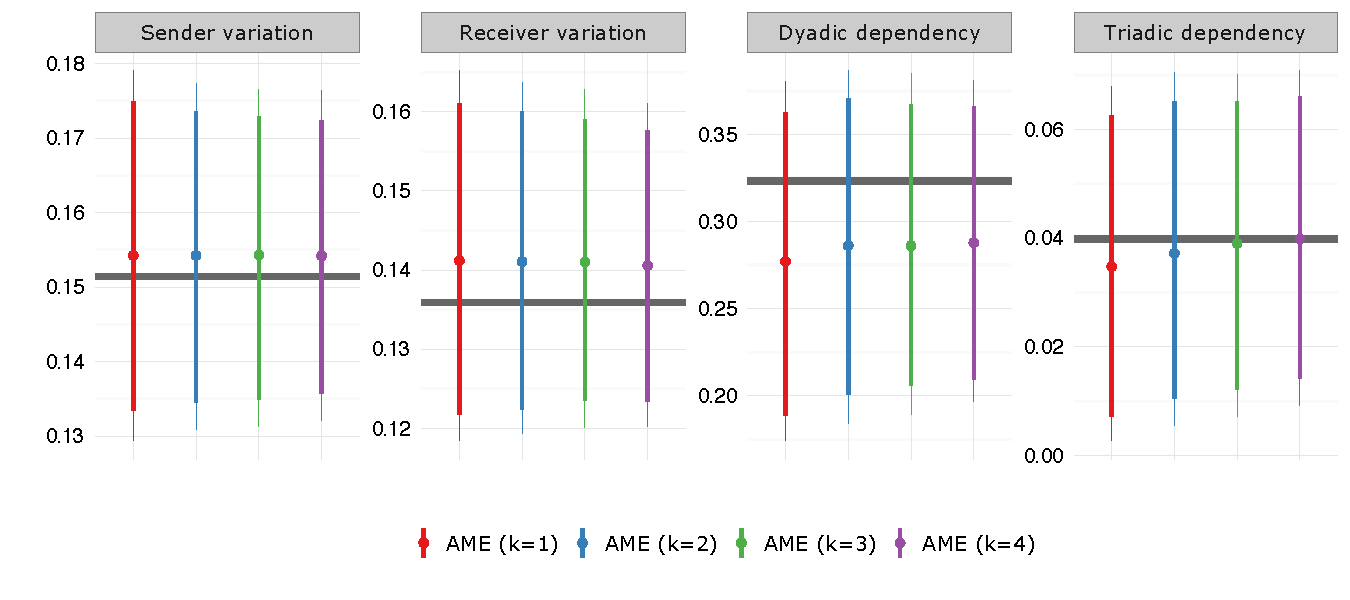
\includegraphics[width=1\textwidth]{netPerfCoef_ameSR}
% 	\caption{Network goodness of fit summary using \pkg{amen}.}
% 	\label{fig:netPerfCoef_ameSR}
% \end{figure}


% Bib stuff
\clearpage
 \bibliography{/Users/mdw/git/whistle/master}
% \bibliography{/Users/janus829/whistle/master}
%\bibliography{/Users/s7m/whistle/master}
\bibliographystyle{elsarticle-harv}\biboptions{authoryear}
\newpage

\end{document} 